\chapter{Design de recherche}

Dans ce chapitre nous présentons la démarche expérimentale que nous avons choisie d{\textquoteright}utiliser pour mener à bien cette recherche, ainsi que les résultats que nous avons obtenus. Nous avons choisi de nous saisir de différents outils informatiques, algorithmiques et de visualisation afin d{\textquoteright}observer les mèmes circulant sur Sina Weibo. Nous débuterons ce chapitre en discutant des implications d{\textquoteright}une méthodologie fondée sur l{\textquoteright}analyse et la visualisation de données pour une recherche en sciences sociales. Dans un second temps, nous brosserons un panorama des méthodes utilisées pour explorer les données issues des réseaux sociaux. Enfin, nous présenterons notre démarche ainsi que les résultats de cette étude. 


\section[Sciences sociales du réseau]{Sciences sociales du réseau}
Pour l{\textquoteright}empiriste, l{\textquoteright}acte essentiel de la recherche est l{\textquoteright}observation. Structure schématique faite de points et de lignes, le réseau n{\textquoteright}offre que peu de prises pour une approche empirique. Pourtant, ce concept protéiforme traverse aujourd{\textquoteright}hui les disciplines pour se retrouver au centre des débats scientifiques. Couplé à l{\textquoteright}autre grand insaisissable de l{\textquoteright}étude qu{\textquoteright}est \textit{l{\textquoteright}information, }le modèle du réseau fait la promesse de nouvelles perspectives en offrant un cadre conceptuel commun pour les sciences et de nouveaux horizons méthodologiques gr\^ace aux outils informatiques. L{\textquoteright}interrogation autour des réseaux se trouve donc plus que jamais au c{\oe}ur du devenir des sciences. 

\subsection[Le réseau comme enjeu pour l{\textquoteright}étude]{Le réseau comme enjeu pour l{\textquoteright}étude}
Durant la seconde guerre mondiale et jusqu{\textquoteright}à la fin des années 1950, les esprits les plus brillants du siècle (G\"odel, Von Neumann, Einstein..) se c\^otoient à \textit{l{\textquoteright}Institut des Etudes Avancées} de Princeton (IAS) aux USA et leurs travaux posent les bases logiques et technologiques d{\textquoteright}o\`u émerge la science informatique actuelle. Dans le domaine de la philosophie mathématique tout d{\textquoteright}abord, les interrogations amorcées par Russel dans ses \textit{Principia Mathematica }puis leur critique par G\"odel dessinent les contours d{\textquoteright}une {\textquotedblleft}machine récursive{\textquotedblright}, anc\^etre mathématique de la machine de Turing et de l{\textquoteright}ordinateur de Von Neumann. Considéré comme le père de l{\textquoteright}ordinateur, Von Neuman s{\textquoteright}exile d{\textquoteright}Allemagne pour rejoindre l{\textquoteright}IAS nouvellement fondé dès 1933 o\`u il poursuit des recherches dans le domaine de la physique nucléaire. En 1943, Von Neumann intègre le \textit{Projet Manhattan} dirigé par Oppenheimer o\`u il est chargé de superviser l{\textquoteright}immense processus de calcul nécessaire à la construction de la bombe qui s{\textquoteright}abattra sur Hiroshima le 6 A\^out 1945. C{\textquoteright}est durant cette période que Von Neumann développe l{\textquoteright}architecture encore utilisée aujourd{\textquoteright}hui comme base fondamentale du design électronique. Dans ses lectures à l{\textquoteright}Université de Yale en 1957 parues sous le titre célèbre de \textit{L{\textquoteright}Ordinateur et le Cerveau} \citep{Neumann1948}, Von Neumann identifie les différentes unités d{\textquoteright}un ordinateur : unité d{\textquoteright}arithmétique logique, unité de contr\^ole, mémoire et entrées/sorties. Les travaux teintés d{\textquoteright}ombre de ce prestigieux mathématicien font écho à ceux de l{\textquoteright}anglais Turing qui travaille également sur la question de l{\textquoteright}intelligence des machines depuis le début de la guerre. Leur correspondance témoigne du respect mutuel qu{\textquoteright}entretiennent alors les deux savants, ainsi que leurs nombreux questionnements sur la possibilité d{\textquoteright}une machine intelligente \citep{Istrail2013}. Au c{\oe}ur de leurs discussions se trouve la qu\^ete d{\textquoteright}un modèle universel capable d{\textquoteright}expliquer le fonctionnement de l{\textquoteright}activité cognitive.  

Norbert Wiener, un autre prodige des mathématiques prend également part à cette recherche. Sa théorie qu{\textquoteright}il nomme \textit{cybernétique }place la notion d{\textquoteright}information au c{\oe}ur de la réflexion sur le fonctionnement des systèmes : \textit{{\textquotedblleft}Information is information, not matter or energy{\textquotedblright}} \citep{Neumann1948}, p. 155). Utilisant les concepts de bruit, de messages et de \textit{feedbacks}, il jongle entre mathématiques appliquées et sciences cognitives pour comprendre les phénomènes de transmission de signaux complexes. Dans une lettre du 29 Novembre 1946, Von Neumann écrit à Wiener que l{\textquoteright}étude du cerveau {\textquotedblleft}\textit{the most complicated object under the sun, litterally}{\textquotedblright} nécessite de poursuivre une réflexion transverse à de multiples disciplines scientifiques \citep{Masani1990}. Depuis le début de cette m\^eme année 1946, les {\textquotedblleft}conférences cybernétiques{\textquotedblleft} aussi connues sous le nom de {\textquotedblleft}conférences Macy{\textquotedblright} ont débuté à New York dans le but de définir \textit{{\textquotedblleft}une science général de l{\textquoteright}esprit humain{\textquotedblright}}\footnote{ Foundation for Cybernetics, The Macy Conferences \url{http://www.asc-cybernetics.org/foundations/history/MacySummary.htm} consulté le 10 Mars 2014 à 16h16 GMT+1}. Regroupant physiciens, cogniticiens, biologistes, anthropologues et linguistes, ces conférences sont l{\textquoteright}objet de nombreuses publications dont \textit{The Human Use of Human Beings} \citep{Wiener1988} qui propose d{\textquoteright}étudier la société en considérant les communications entre hommes et machines. Le travail mené lors de ces conférences est souvent considéré comme la pierre fondatrice du champ des études sur la communication \citep{Breton1997, Winkin1981}. Quelques années plus tard, McLuhan et son idée controversée de \textit{village global} \citep{McLuhan1962} amènent un large auditoire autour des {\oe}uvres de Wiener et l{\textquoteright}étude des modes de communication. Progressivement se constitue un champ épistémologique pour l{\textquoteright}étude de l{\textquoteright}information dont la définition reste encore aujourd{\textquoteright}hui un enjeu important \citep{Wolton1997}. En France, les Sciences de l{\textquoteright}Information et de la Communication se sont principalement structurées autour de la critique des médias \citep{Mattelart1986, Debray1991} dans une tradition européenne déjà bien installée \citep{Adorno2005}. Aux Etats-Unis, les \textit{cultural studies }\citep{Hall2003} s{\textquoteright}interrogent davantage sur l{\textquoteright}économie politique des symboles et trouvent leurs lettres de noblesse dans les \textit{media studies, }aujourd{\textquoteright}hui devenue une discipline universitaire reconnue en Angleterre et aux USA. Toutefois, l{\textquoteright}émergence d{\textquoteright}un \textit{{\textquotedblleft}paradigme communicationnel{\textquotedblright} }\citep{Bougnoux1993} nécessite un dialogue pas toujours évident entre les différentes disciplines constituées autour de l{\textquoteright}étude des pratiques de l{\textquoteright}information et de la communication : sociologie des médias, études des systèmes d{\textquoteright}information, informatique, sciences de l{\textquoteright}information et de la communication, etc.  


Alors que le programme fixé par la cybernétique a pour ambition  d{\textquoteright}explorer les structures, possibilités et  contraintes des systèmes communicants, l{\textquoteright}image  fermée et cyclique du système devient rapidement trop étriquée  pour une réflexion sur les relations en pleine expansion. Deleuze et  Guattari proposent dans l{\textquoteright}introduction de leur livre  \textit{Milles Plateaux} \citep{Deleuze1972} de s{\textquoteright}éloigner de  l{\textquotesingle}arborescence classique du système auto-suffisant  pour envisager les liens entre sujets et objets sous la forme ouverte  et combinatoire du \textit{rhizome. }Le rhizome se définit par son  caractère non-fini et fait de l{\textquoteright}étude des  causalités un phénomène contextuel aux spécificités pas  forcément reproductibles. Imperméable à la catégorisation et  aux classifications ordonnées, l{\textquoteright}objet  d{\textquoteright}étude in-formé devient \textit{open-ended},  moment donné à voir et état unique d{\textquoteright}un ensemble  plus vaste. La vérité ou la validité n{\textquoteright}est donc  plus à découvrir dans l{\textquoteright}analyse, mais plut\^ot dans  l{\textquoteright}articulation des contingences entre objets et  environnements dont se saisit le champ émergent des études sur la  complexité \citep{Morin1990}. Dans le m\^eme temps, les progrès de  l{\textquoteright}intelligence artificielle et de la robotique viennent  également questionner notre définition du vivant face à ces  nouveaux \^etres \citep{Hofstadter1999}. Le modèle du \textit{réseau  }vient à son tour in-former la pensée scientifique comme un nouvel  \textit{episteme }foucaldien offrant une grille de lecture des faits  sociaux renouvelée \citep{Castells1989, Latour1996}.  Aujourd{\textquoteright}hui, la structuration d{\textquoteright}un  champ de recherche cohérent et multi-disciplinaire autour de  l{\textquoteright}étude des réseaux reste un enjeu important pour  le monde de la recherche \citep{Brandes2013}. Cette considération  pour la complexité des phénomènes permet en effet  d{\textquoteright}imaginer une approche scientifique qui atténuerait  les liens entre des disciplines dont le dialogue parfois difficile est  néanmoins nécessaire, afin de mener vers une réconciliation des  sciences humaines, des sciences naturelles et des sciences du vivant  o\`u cohabiteraient  \textit{{\textquotedblleft}l{\textquoteright}étude des organismes, des organes et des organisations{\textquotedblright} }\citep{Morin1990}


\subsection[Code, données et les nouveaux outils de l{\textquoteright}écriture scientifique ]{Code, données et les nouveaux outils de l{\textquoteright}écriture scientifique }
Les objets ouverts et mal définis du réseau posent néanmoins la question d{\textquoteright}une continuité avec le projet aristotélicien d{\textquoteright}une compréhension du monde par le savoir analytique. La considération d{\textquoteright}un objet comme moment du réseau rend caduque l{\textquoteright}idée de sa définition \textit{a priori, }en dehors des relations qu{\textquoteright}il entretient avec son environnement. A l{\textquoteright}inverse, une définition des objets entre origine, fonction et destination ne devrait pas éluder non plus la réflexion ontologique autour de son \textit{\^etre}. Le philosophe américain William James propose une méthode qu{\textquoteright}il nomme \textit{empirisme radical }o\`u l{\textquoteright}existence des objets doit \^etre considérée par le prisme de l{\textquoteright}expérience \citep{James1912}\textit{. }L{\textquoteright}expérience, m\^eme scientifique, existe dans un contexte, un lieu, un temps, un moment, une succession d{\textquoteright}étapes, et c{\textquoteright}est cet ensemble qui nous permet de percevoir les phénomènes étudiés. Si l{\textquoteright}acte essentiel de l{\textquoteright}empiriste et du philosophe est l{\textquoteright}observation, alors elle doit \^etre radicale dans son honn\^eteté et accepter l{\textquoteright}expérience dans son unicité dont de nombreux facteurs sont non-reproductibles. Cette question de l{\textquoteright}expérience et de sa reproductibilité est depuis toujours au c{\oe}ur du débat sur les sciences et se pose comme un des ressorts fondamentaux du savoir scientifique. Les sciences dites {\textquotedblleft}dures{\textquotedblright} comme la physique, la biologie, l{\textquoteright}informatique ou m\^eme la géologie valident leurs hypothèses gr\^ace à l{\textquoteright}usage extensif d{\textquoteright}appareillages multiples devenus une clé de la reproductibilité des expériences. Du simple microscope à l{\textquoteright}accélérateur du CERN, la méthodologie d{\textquoteright}observation est pour ces disciplines souvent indissociable de la technologie. Le travail de la recherche et de la preuve s{\textquoteright}articule ici autour des trois p\^oles de la théorie, de l{\textquoteright}expérience et de la méthode conditionnée à la technique.  

\begin{figure}
    \centering
    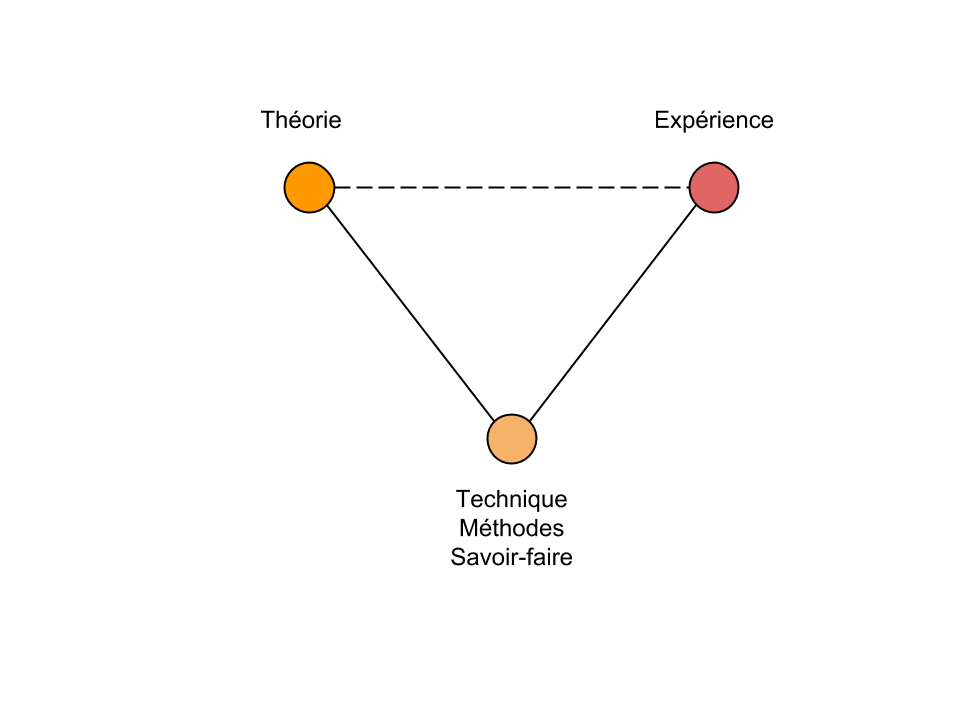
\includegraphics[width=5.0559in,height=3.7894in]{figures/chap3/chapitre3-img1.png}
    \caption[Triptyque des pratiques scientifiques]{Triptyque des pratiques scientifiques}
\end{figure}


En sciences sociales néanmoins, la tension entre la théorie (les concepts), l{\textquoteright}expérience (le terrain) et la méthodologie s{\textquoteright}articule plus rarement autour d{\textquoteright}outillages élaborés. Les \ réflexions sur la méthodologie en sciences sociales portent plus largement sur des argumentations conceptuelles o\`u le langage lui-m\^eme est considéré comme l{\textquoteright}outil premier ou encore de nombreuses réflexions éthiques sur l{\textquoteright}impact des pratiques d{\textquoteright}observation dans le cadre de l{\textquoteright}anthropologie notamment. En France, l{\textquoteright}intér\^et constant porté à l{\textquoteright}utilisation des différentes formes de technologie en sciences humaines s{\textquoteright}est souvent constitué autour de la critique de méthodologies quantitatives très répandues outre atlantique - la statistique en sociologie, l{\textquoteright}étude comportementaliste en psychologie ou le film ethnographique \citep{Becker1996}. Comme le note justement Latour, la qu\^ete de légitimité des Sciences Sociales s{\textquoteright}est souvent traduit par une capacité à se procurer et traiter des données : \textit{{\textquotedblleft}Sociology has been obsessed by the goal of becoming a quantitative science.{\textquotedblright}} \citep{Latour2003}. Pourtant, il serait illusoire de corréler la quantité de données à une quelconque objectivité de la démarche scientifique, tant les démarches et outils nécessaires pour la collecte sont en soi autant de biais importants. La question de la réussite des études utilisant les Big Data semble davantage corrélée à la capacité d{\textquoteright}une approche méthodologique forgée dans un échange interdisciplinaire et des pratiques renouvelées de l{\textquoteright}écriture. La complexité des questions abordées lors du traitement des données, non seulement technologique mais aussi dans les interrogations sur la légitimité de leur existence, leur utilisation et leur provenance \citep{Boyd2011} rendent nécessaire la discussion entre de multiples connaissances. Aujourd{\textquoteright}hui, l{\textquoteright}utilisation de l{\textquoteright}ordinateur conditionne l{\textquoteright}écriture scientifique de l{\textquoteright}étude de terrain, la prise de notes, la rédaction ou la publication et se présente ainsi comme un impératif méthodologique pour la réflexion et le travail en sciences humaines et sociales \citep{Wieviorka2013}. L{\textquoteright}appareillage projeté au centre de la pratique quotidienne du chercheur vient modifier le travail de réflexion sur les phénomènes étudiés et s{\textquoteright}accompagne de multiples contraintes. La prise en main de ce nouvel \textit{{\textquotedblleft}instrument intellectuel{\textquotedblright} }\citep{Guichard2014} passe par une lente alphabétisation aux langages des machines. L{\textquoteright}angoisse latente du {\textquotedblleft}bug{\textquotedblright} n{\textquoteright}est pas apaisée par les rares techniciens présents dans les centres de recherche en sciences humaines, souvent déjà dépassés par la diversité des demandes technologiques. L{\textquoteright}écriture, savoir-faire indispensable de la recherche, possède une nouvelle matérialité dans les disques durs produisant une dépendance accrue aux réseaux d{\textquoteright}ordinateurs. Cette empreinte {\textquotedblleft}digitale{\textquotedblright} laissée par les calculateurs sur les pratiques scientifiques n{\textquoteright}est ni anodine ni révolutionnaire et s{\textquoteright}inscrit dans la longue tradition des cultures de l{\textquoteright}écrit qui déjà bien avant les moines copistes \textit{{\textquotedblleft}combinent les gestes de la main et les opérations de la pensée.{\textquotedblright}} \citep{Jacob2011}  

Tim Berners-Lee, considéré comme l{\textquoteright}inventeur du World Wide Web et du Web Sémantique définit la constitution d{\textquoteright}un réseau mondial des savoirs comme un projet d{\textquoteright}\textit{{\textquotedblleft}ingénierie philosophique{\textquotedblright} }\citep{Halpin2014}. Mi-philosophe mi-ingénieur, le chercheur contribuant à ce réseau de savoir doit donc \^etre en capacité de conna\^itre les protocoles et les langages pour y accéder et s{\textquoteright}y mouvoir aisément. La méthode scientifique s{\textquoteright}écrit notamment avec de nouvelles formulations (fonctions, algorithmes, code...). Les données générées par les usages d{\textquoteright}un nombre croissant de machines communicantes et productrices d{\textquoteright}information, souvent désignées par le concept {\guillemotleft} valise {\guillemotright} de Big Data \citep{Lohr2012} offrent des possibilités nouvelles pour l{\textquoteright}étude en sciences sociales. L{\textquoteright}analyse de ces vastes jeux de données s{\textquoteright}accompagne également de nouveaux impératifs et questionnements sur l{\textquoteright}observation des phénomènes humains qu{\textquoteright}ils représentent. à la fois barrière et opportunité, une difficulté majeure réside dans le discernement nécessaire entre praxis des outils informatiques, fascination pour ces outils et réflexions pertinentes sur la qualité des méthodes employées. Le traitement quantitatif par ordinateur permet d{\textquoteright}extraire de nombreuses connaissances utiles de jeux de données parfois très importants mais n{\textquoteright}assure pas pour autant la qualité des résultats. Une bonne compréhension de la provenance et des méthodes de collection des données est nécessaire afin d{\textquoteright}identifier des algorithmes de traitements intéressants, adaptés et efficaces parmi ceux disponibles \citep{Rajaraman2011}. Les méthodologies d{\textquoteright}exploration et de recherche utilisant le {\textquotedblleft}Big Data{\textquotedblright} comme source nécessitent la mise en {\oe}uvre d{\textquoteright}une ingénierie complexe soutenue par une connaissance des technologies nécessaires à l{\textquoteright}analyse de données. L{\textquoteright}algorithmique, la statistique, l{\textquoteright}informatique mais également la cartographie et le design graphique doivent se conjuguer pour permettre de produire des résultats à la fois intéressants et fiables. Ce travail d{\textquoteright}hypothèses et de vérifications pour l{\textquoteright}analyse de données doit réunir de nombreuses compétences. La définition de la problématique la plus adaptée nécessite une connaissance aig\"ue du terrain et des outils et algorithmes qui seront articulés au sein d{\textquoteright}un système ingénierique parfois très complexe. Le design et la lecture d{\textquoteright}algorithme pour le \textit{{\textquotedblleft}data mining{\textquotedblleft}} sont donc les clés pour le travail du chercheur confronté aux données. Néanmoins, ces algorithmes ne devraient \^etre que la traduction de questions formulées gr\^ace à une connaissance aig\"ue des problématiques du contexte et des objets étudiés - notamment pour identifier les données manquantes. La {\textquotedblleft}science des données{\textquotedblright} promet donc d{\textquoteright}apporter un véritable renouveau des méthodes et des résultats scientifiques, au prix d{\textquoteright}un travail soutenu pour faire face à ces changements d{\textquoteright}habitudes et de langages. Les applications statistiques du {\textquotedblleft}big data{\textquotedblright} permettent aujourd{\textquoteright}hui une fiabilité accrue des prédictions par l{\textquoteright}augmentation du volume des corpus traités \citep{Breiman2001}. Le domaine de l{\textquoteright}intelligence artificielle (AI) a grandement bénéficié de l{\textquoteright}accroissement de la capacité de traitement des données notamment pour la prédiction gr\^ace au techniques dites de \textit{machine learning}. Néanmoins Peter Norvig, directeur de recherche chez Google, reconnait lui-m\^eme : {\textquotedblleft}\textit{We could draw this curve: as we gain more data, how much better does our system get? And the answer is, it{\textquoteright}s still improving---but we are getting to the point where we get less benefit than we did in the past.{\textquotedblright} }\citep{Somers2013}. Comme le note Douglas Hofstadter, un des pairs de l{\textquoteright}Intelligence Artificielle à propos du super-ordinateur qui venait de battre Kasparov aux échecs : \textit{{\textquotedblleft}Okay, Deep Blue plays very good chess---so what? Does that tell you something about how we play chess? No. Does it tell you about how Kasparov envisions, understands a chessboard?{\textquotedblright} }\citep{Somers2013}.  

En effet, ces pratiques méthodologiques doivent réussir à s{\textquoteright}inscrire dans la continuité de l{\textquoteright}historicité et des exigences des disciplines. La portabilité des méthodes et la disponibilité des données sont encore des questions centrales et non-résolues. En sciences sociales notamment, les services de réseaux sociaux en ligne offrent de très larges corpus dont l{\textquoteright}utilisation est régie par les exigences commerciales des sociétés privées qui les détiennent. L{\textquoteright}analyse des données issues de service de réseaux sociaux en ligne est pourtant un champ d{\textquoteright}études en rapide expansion \citep{Nettleton2013}. Pourtant, le débat sur la validité des éclairages apportés par l{\textquoteright}analyse des données issues des services de réseaux reste encore largement ouvert et nous entendons dans ce travail de recherche y contribuer.  

\subsection[Visualisation et espace perceptif pour l{\textquoteright}information]{Visualisation et espace perceptif pour l{\textquoteright}information}

Face à de larges volumes de données, un des grands enjeux est d{\textquoteright}en restituer une forme intelligible afin d{\textquoteright}identifier des tendances ou des motifs particuliers. La visualisation permet de produire une lecture particulière de parties intéressantes et intelligibles d{\textquoteright}un jeu de données \citep{Cairo2013}. Définie comme \textit{{\guillemotleft}~a process that transforms data, information, and knowledge into a form that relies on the human visual system to perceive its embedded information.{\textquotedblright}} \citep{Graffieti2010}, la visualisation introduit la question du design visuel au c{\oe}ur de la problématique d{\textquoteright}analyse \citep{Wesolowsky1992}. La visualisation correspond à une série d{\textquoteright}actions qui résulte dans la production de marqueurs visuels (points, ligne, aires, surface, volume) avec comme étapes la définition de leurs propriétés rétiniennes (couleur, taille, texture, etc.) et leur positionnement dans l{\textquoteright}espace visuel \citep{Card1997}. Dans son travail, Engelhardt \cite{Engelhardt2007} s’attache   à définir les bases d{\textquoteright}une grammaire de la visualisation en commen\c{c}ant par en identifier les formes syntaxiques :  
\begin{enumerate}
\item les objets graphiques montrés (ex. point, flèche, pictogramme, etc.), 
\item l{\textquoteright}espace graphique donnant sens à l{\textquoteright}organisation des objets (ex. systèmes de coordonnnées géographiques, timeline, etc.), 
\item les propriétés graphiques des objets (couleurs, tailles, etc.), 
\item l{\textquoteright}organisation des objets en différentes catégories (ex. cadre, liens, légendes, etc.). 
\end{enumerate}

Ces choix forment une t\^ache importante dont l{\textquoteright}enjeu n{\textquoteright}est pas seulement visuel, mais se joue également dans le champ de la représentation o\`u les objets sont donnés à voir et par là-m\^eme donnés à comprendre. Les travaux sur l{\textquoteright}apparition de la perspective dans la Renaissance italienne ont montré comment l{\textquoteright}espace de la représentation visuelle fait écho aux changements sociétaux profonds de l{\textquoteright}époque \citep{Raynaud2005}. Au-delà d{\textquoteright}une simple technique picturale, les {\oe}uvres des peintres du Quattrecento témoignent de changements profonds dans la perception : l{\textquoteright}espace perceptif se structure désormais autour du sujet et \ de son {\textquotedblleft}point de vue{\textquotedblright} qui construit l{\textquoteright}ensemble de la représentation \citep{Damisch1999}. Empreinte de rationalité, la perspective construit comme au thé\^atre un espace de représentation centré autour du spectateur. En 1639, le mathématicien Desargues modélise les notions intuitives de perspective et d{\textquotesingle}horizon gr\^ace à la géométrie projective qui permet d{\textquoteright}étudier les propriétés inchangées des figures lors de leur projection. Cette géométrie d{\textquoteright}un genre nouveau se structure autour du \textit{plan projectif}, élément topologique qui \textit{{\textquotedblleft}rassemble en une seule surface l{\textquoteright}imagination de tous les points de vue possible{\textquotedblright} }\citep{Petit1999}. En construisant un plan géométrique fondé sur le point de vue, de nouveaux \^etres géométriques aux propriétés étranges voient le jour, dont l{\textquoteright}existence logique force notre représentation classique : la bande de M\"obius ne possède qu{\textquoteright}une seule face et il est impossible de distinguer l{\textquoteright}intérieur de l{\textquoteright}extérieur d{\textquoteright}une bouteille de Klein. Dans ces surfaces dites \textit{unilatères}, le local est traversé en tout point par un tout global. Nous ne pouvons pas traverser puisque nous somme toujours sur la m\^eme face. Ni bord, ni extérieur, ni intérieur, le plan projectif apporte des éléments de réponses conceptuelles aux limites des la représentation dans l{\textquoteright}espace.

Dans le contexte de systèmes et de réseaux complexes, la visualisation de données structure l{\textquoteright}espace perceptif afin de construire une scène à \textit{n }dimensions dont l{\textquoteright}enjeu est la recherche d{\textquoteright}un {\textquotedblleft}point de vue{\textquotedblright} pour l{\textquoteright}étude\textit{. }Alors que la perspective prend pour parti de matérialiser le sujet au centre de la représentation par des points de fuite, la visualisation de données cherche elle à utiliser les objets comme dimensions du champ de la représentation, en structurant souvent l{\textquoteright}espace autour de quantités. Néanmoins, la place du spectateur / utilisateur dans la visualisation reste un des enjeux majeurs encore à explorer. En élaborant sa {\textquotedblleft}méthode graphique{\textquotedblright} , J.E. Marey \citep{Marey1885} utilise la photographie pour créer un nouvel espace de représentation du mouvement et observer des phénomènes jusqu{\textquoteright}ici invisibles. Si la temporalité de l{\textquoteright}écrit ou de la voix est avant linéaire, l{\textquoteright}espace visuel permet de manier le réel pour le décomposer en actes logiques. Charcot cherche dans les images de l{\textquoteright}hystérie des témoignages de la folie et procède à la mise en scène de ses patients dans ce nouvel espace de représentation ouvert par la photographie \citep{DidiHuberman2012}.

La visualisation scientifique se prévaut donc d{\textquoteright}une existence avant tout pratique dont le premier objectif serait de \textit{{\guillemotleft}~to effectively convey information~{\guillemotright}} \citep{Kelleher2011}. Son caractère syncrétique et sa capacité à résumer une large masse d{\textquoteright}information rapidement en font un des plus importants éléments de la publication en science notamment pour sa diffusion et la facilitation d{\textquoteright}accès à une connaissance \citep{Ware2004}. Dans sa sémiologie graphique, Bertin \citep{Bertin1977} distingue deux usages majeurs des graphiques de visualisation : 1) un moyen de communiquer des informations (dans le cas o\`u l{\textquoteright}information a déjà été comprise) 2) un moyen visuel de résoudre des problèmes logiques (quand le graphique est utilisé comme support de lecture et de manipulation d{\textquoteright}informations). Ces deux caractéristiques peuvent coexister dans certaines pièces mais la transition entre les deux nécessite souvent un travail important de restructuration visuelle. Dans le traitement et la visualisation des données \textit{l{\textquoteright}interface }joue un r\^ole primordial. On peut désormais agir sur la deuxième catégorie de Bertin pour mieux explorer le sens \citep{Weissberg2007}. Manovich montre comment l{\textquoteright}interface définie comme \textit{{\textquotedblleft}the ways to represent ({\textquoteleft}format{\textquoteright}) and control the signal.}{\textquotedblright} \citep{Manovich2013}. Ce formatage nouveau de l{\textquoteright}information induit des changements dans la pratique de la lecture qui, toujours selon Manovich, s{\textquoteright}apparenterait davantage à de la reconnaissance de \textit{pattern}, symbolisé par l{\textquoteright}usage de l{\textquoteright}ic\^one et du menu en design d{\textquoteright}interface. Ainsi si l{\textquoteright}interface contraint la lecture, la prise en compte des formes narratives (les \textit{patterns} de Manovich) prend une grande importance quand il s{\textquoteright}agit de concevoir une visualisation d{\textquoteright}information. L{\textquoteright}usage des signes graphiques doit se faire avec une connaissance des usages de l{\textquoteright}interface, afin de recréer la coopération textuelle des r\^oles de lecteur et de designer/auteur nécessaire pour la production un sens \citep{Eco1985}. La \textit{citizen science} ou encore \textit{night science} a fait de l{\textquoteright}interface un paradigme en utilisant la visualisation pour amener un grand nombre de collaborateurs à explorer et analyser de vastes jeux de données en effectuant des t\^aches simples \citep{Silvertown2009}. Le projet \textit{Eyewire} permet à des internautes de contribuer à la classification d{\textquoteright}images du cerveau humain en vue de la réalisation d{\textquoteright}un modèle 3D \citep{Seung2012}. Utilisant des scans de tranches de 1mm réalisés par l{\textquoteright}institut Max Planck, la modélisation 3D d{\textquoteright}un cerveau complet promet une belle contribution pour la découverte des fonctionnements cognitifs. Néanmoins, la t\^ache est colossale et nécessiterait plusieurs années pour une équipe classique de scientifiques. \textit{Eyewire} propose donc une interface web o\`u un simple jeu de coloriage permet d{\textquoteright}identifier les neurones et de contribuer ainsi au dessin du modèle 3D.

Cartes, code ou graphiques, les nouveaux outils numériques participent donc à structurer de nouvelles pratiques de l{\textquoteright}espace numérique gr\^ace à la construction de nouvelles représentations. 

\section[L{\textquoteright}analyse de la diffusion sur les réseaux sociaux]{L{\textquoteright}analyse de la diffusion sur les réseaux sociaux}

Nous allons maintenant regarder comment l{\textquoteright}analyse des données des services de réseaux sociaux en ligne (SNA) peut permettre d{\textquotesingle}interroger les pratiques des technologies numériques pour mieux en comprendre les tenants. 


\subsection[Anatomie d{\textquoteright}un réseau social]{ Anatomie d{\textquoteright}un réseau social}

La représentation des relations sociales sous forme de graphe trouve son origine dans les travaux des psychologues allemands de la \textit{gestalt }durant les années 1920-1930 \citep{Scott1988}\textit{. }S{\textquoteright}inspirant des études sur le cerveau, le psychologue J. L. Moreno s{\textquoteright}applique notamment à comprendre les principes organisationnels holistiques des groupes humains et fonde la sociométrie avec comme objectif la qualification et la quantification des relations sociales \citep{Moreno1938}. Moreno cherche à identifier et isoler des leaders de groupes sociaux définis en étudiant l{\textquoteright}asymétrie ou la réciprocité de leurs choix et fréquentations amicales. Cherchant des moyens de représenter les tendances à l{\textquoteright}auto-organisation qu{\textquoteright}il observe, il cartographie les relations directes et indirectes entre personnes sous forme de \textit{sociogrammes}. Les anthropologues s{\textquoteright}emparent rapidement de ce type d{\textquoteright}outils pour comprendre les formes tribales (Lundberg, 1936) et l{\textquoteright}émergence progressive de la topologie comme domaine important des mathématiques vient définir de nouveaux types de relations entre objets disparates, avec notamment la théorie des graphes qui donne à l{\textquoteright}étude des réseaux ses modèles logiques \citep{Harary1977}. Milgram \citep{Travers1969} voit les relations humaines comme autant de petits mondes (\textit{small-worlds)} connectés entre eux. Granovetter s{\textquoteright}intéresse à l{\textquoteright}importance des relations ténues et lointaines (\textit{weak ties}) dans l{\textquoteright}acquisition d{\textquoteright}informations importantes \citep{Granovetter1973}. L{\textquoteright}influence de la théorie des graphes amène notamment les sociologues à expérimenter de nouveaux modèles venus de la physique ou de la biologie, en proposant de nouvelles pratiques comme celle de la simulation sociale \citep{Epstein1996}. 


La matérialité de l{\textquoteright}image du \textit{graphe} structure la représentation du réseau social. Dans la littérature concernant les réseaux, les notions de graphe et de réseau sont interdépendantes et la théorie des graphes sert notamment de systèmes de notation pour la mise en équation des réseaux \citep{Nettleton2013}. Si cette structure point-ligne semble toutefois rev\^etir une limite de taille pour la description de phénomènes humains (comment en effet réduire les relations humaines à une simple ligne?), elle semble néanmoins aujourd{\textquoteright}hui encore difficile à dépasser.

\begin{figure}
    \centering
    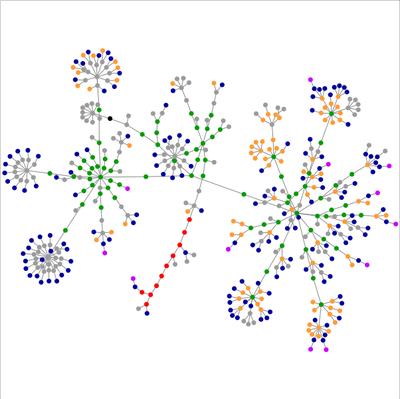
\includegraphics[width=4.178in,height=4.1449in]{figures/chap3/chapitre3-img2.png}
    \caption{Représentation d'un réseau sous forme de graphes.}
\end{figure}


Un réseau considéré comme graphe, noté \textit{G}, se compose d{\textquoteright}un ensemble de nodes ou vertices (les points) et de liens ou edges (les traits). On représente ainsi un graphe sous la notation \textit{G(V,E)} o\`u \textit{V }est l{\textquoteright}ensemble des nodes du réseau et \textit{E} l{\textquoteright}ensemble des liens\textit{ }décrivant leurs relations. \textit{E }décrit les relations entre les nodes qui peuvent \^etre directionnelles (paires de vertices ordonnées) dans le cas d{\textquoteright}un graphe \textit{orienté }ou accompagné de valeurs particulières dans un graphe dit \textit{pondéré. }Les relations ainsi exprimées portent sur un aspect unique, quantifiable et isolable. La prise en compte de facteurs multiples, comme notamment l{\textquoteright}espace physique, le temps, mais également les multiples réseaux de relations qui peuvent exister entre deux acteurs nous amènent à considérer un graphe disposant de multiples couches \textit{(}\textit{multi-layered)} pour décrire l{\textquoteright}ensemble des groupes de relations. Imaginons un graphe de personnes \textit{G (V,E}\textit{\textsubscript{n}}\textit{)} o\`u \textit{V }sont les vertices représentant les personnes et \textit{E}\textsubscript{n} un nombre \textit{n }d{\textquoteright}ensemble de liens\textit{ }décrivant chaque type de relations spécifiques. Le graphe ci-dessous montre un exemple d{\textquoteright}un graphe multi-couche o\`u \textit{E}\textit{\textsubscript{1}} est l{\textquoteright}ensemble des relations amicales, \textit{E}\textit{\textsubscript{2}}\textsubscript{ }les relations de travail et \textit{E}\textit{\textsubscript{3}}\textsubscript{ }les relations familiales.

\begin{figure}
    \centering
    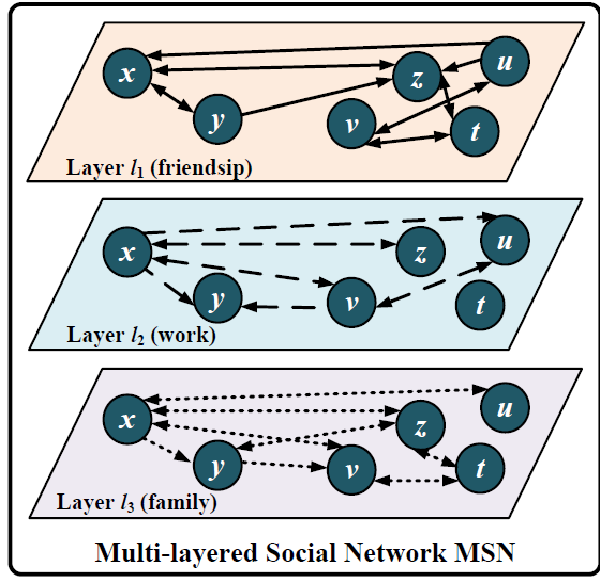
\includegraphics[width=3.8004in,height=3.6894in]{figures/chap3/chapitre3-img3.png}
    \caption [réseau social multi-couches] {Un réseau social multi-couches, d{\textquoteright}après (Brodka\&al., 2013)}
\end{figure}

Nous pouvons ainsi décrire différents jeux de relations entre un jeu d{\textquoteright}acteurs finis, permettant notamment de mieux comprendre les relations entre ses différentes dimensions. Si cette approche résout momentanément la question des \textit{n }dimensions à considérer \citep{Brodka2013} elle augmente également la complexité du graphe et la possibilité d{\textquoteright}erreurs de lecture ou de typage des relations.

Afin de mieux comprendre l{\textquoteright}organisation d{\textquoteright}un réseau, nous disposons de plusieurs mesures~pour décrire les relations et le r\^ole des différents acteurs :

\begin{itemize}
\item \textit{Degree} : (\textit{degré} ou \textit{valence}) mesure le nombre de connections d{\textquoteright}un n{\oe}ud dans un réseau. Cette valeur indique souvent une possibilité, le potentiel d{\textquoteright}un node donné à interagir avec d{\textquoteright}autres.  
\item \textit{Closeness : }(proximité) mesure la facilité d{\textquoteright}un node à se connecter à un autre. Dans un réseau en ligne, on calcule la proximité en estimant la distance la plus courte entre un node et un autre. 
\item \textit{Betweenness} (\textit{centralité}) mesure le degré d{\textquoteright}importance d{\textquoteright}un node dans le réseau en prenant en compte le nombre de nodes dépendant de lui pour
établir une connection entre eux. La centralité représente la capacité à bloquer ou laisser filtrer l{\textquoteright}accès à certaines parties du réseau. Dans une entreprise par exemple, la secrétaire du CEO a par exemple une très haute centralité.
\end{itemize}

En observant ces différentes mesures, nous pouvons définir différentes structures types pour chaque réseau. La distribution des degrés dans le graphe permet notamment de comprendre les modèles qui régissent les connexions entre les nodes. L{\textquoteright}exemple le plus simple est le \textit{random network, }réseau o\`u les acteurs sont connectés de manière entièrement aléatoire. Un réseau dont le degré de distribution correspond à une loi de puissance est appelé \textit{scale-free network. }Un réseau dont seulement quelques nodes possèdent une centralité élevée et dont la structure d{\textquoteright}ensemble est faite de groupes ou \textit{clusters} interconnectés et appelé un \textit{small-world network}.

\begin{figure}
    \centering
    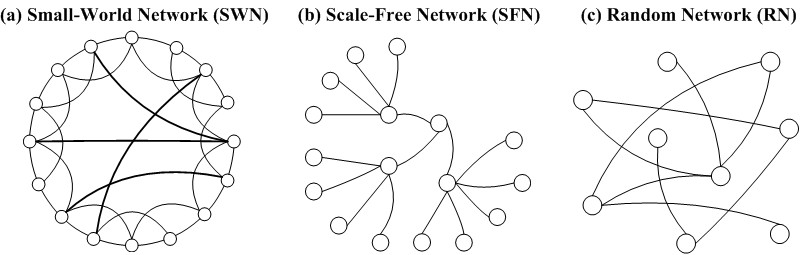
\includegraphics[width=6.3449in,height=2.0224in]{figures/chap3/chapitre3-img4.jpg}
    \caption{Types communs de réseaux}
\end{figure}

Les services de réseaux sociaux en ligne sont structurés en \textit{small-worlds}. Dans une étude analysant de larges corpus issus de différents services de réseaux sociaux en ligne, Kumar \& al. \citep{Kumar2006} ont montré que ces communautés possèdent toutes une structure et une évolution similaire. Les inscrits de chaque service se répartissent autour de trois grands groupes : \textit{singletons} (membres isolés, inactifs), \textit{giant component} (la majorité des utilisateurs actifs) et \textit{middle region} (des communautés isolées qui interagissent entre elles mais pas avec le reste du réseau). D{\textquoteright}après les auteurs, il existe très peu de chances que deux communautés isolées m\^eme très similaires se rencontrent dans ce type de réseau, car l{\textquoteright}entropie de la structure \textit{small-world }se renforce avec le temps en se fragmentant davantage. Une des raisons principales est que ces communautés isolées suivent souvent un modèle en \textit{étoile, }c{\textquoteright}est à dire qu{\textquoteright}elles sont construites autour d{\textquoteright}un individu central charismatique. éventuellement, il leur arrive de rejoindre la masse du \textit{giant component} mais elles en deviennent difficilement des acteurs majeurs et restent en périphérie. Dans un réseau social de type small-world comme les OSNS, les acteurs les plus influents sont ceux qui sont capables de 1) renforcer les liens dans un cluster (\textit{closure)} et 2) développer les connections faibles entre des clusters (\textit{brokerage)} (Burt, Centola, \& Kahl, 2008). Ce {\textquotedblleft}capital social{\textquotedblright} est inscrit dans la structure du réseau social lui-m\^eme \citep{Lin1999} et n{\textquoteright}a pas de relations avec le degré du node (son nombre de connections) \citep{Cha2010}. L{\textquoteright}individu le plus puissant d{\textquoteright}un réseau est donc celui possédant le plus grand nombre de connections \textit{potentielles, }proches et facilement accessibles et qui bénéficie d{\textquoteright}une place privilégiée pour bloquer ou autoriser l{\textquoteright}accès aux autres parties du réseau. L{\textquoteright}analyse organisationnelle a notamment montré l{\textquoteright}importance capitale des secrétaires pour le maintien d{\textquoteright}une bonne circulation des informations dans le réseau de l{\textquoteright}entreprise ou la nécessité d{\textquoteright}un nombre très faible de connections directes pour les acteurs importants de réseaux terroristes ou mafieux \citep{Russel2011}.


\subsection[Analyse de réseaux sociaux et de la diffusion d'information en ligne]{Analyse des réseaux sociaux et de la diffusion d'information en ligne}

L{\textquoteright}analyse de réseau social permet de comprendre la structure d{\textquoteright}un moment du réseau. En effet, les connections entre différents acteurs sont sans cesse en mouvement et l{\textquoteright}information en circulant vient modifier l{\textquoteright}activité du réseau et bien souvent sa structure m\^eme. Notre étude porte sur la diffusion de mèmes au sein du réseau social chinois Sina Weibo et s{\textquoteright}inscrit ainsi dans la continuité des travaux s{\textquoteright}intéressant aux rapports entre diffusion et technologies. Néanmoins, le champ de la diffusion de l{\textquoteright}innovation, objet traditionnel de la géographie, s{\textquoteright}est largement constitué autour des problématiques technologiques et organisationnelles liées à la situation spatiale du lieu et ses équipements \citep{Crevoisier2004}. Les études urbaines ont notamment montré comment la réalité économique et géographique présidait à la constitution des savoirs nécessaires à la diffusion de l{\textquoteright}innovation technologique \citep{Howells2002}. Cette vision doit \^etre modérée par une considération plus importante des modalités d{\textquoteright}appropriation des technologies comme pratiques propres aux territoires \citep{Fernandez2010}. Plus largement, les études sur la diffusion sont dominées par l{\textquoteright}analogie du virus comme modèle de propagation des messages, comportements et idées. Depuis la fin du XIXe siècle \citep{LeBon1895}, ce modèle est prépondérant dans les recherches autour de la diffusion d{\textquoteright}information en ligne \citep{Goel2012} Les membres de groupes dans un réseau seraient \textit{exposés }à un message ou une idée avant d{\textquoteright}\^etre \textit{infectés, }devenant alors porteur puis agent de sa diffusion. Ainsi, en considérant la position d{\textquoteright}un individu au sein du réseau de diffusion, il serait possible de définir un \textit{{\textquotedblleft}}\textit{degré d{\textquoteright}infection{\textquotedblright}} \citep{Cheng2013} et d{\textquoteright}anticiper la diffusion selon une \textit{{\guillemotleft}~probabilité immune~{\guillemotright} }qui\textit{ }déciderait de la \textit{{\guillemotleft}~qualité infectieuse~{\guillemotright} }de l{\textquoteright}objet diffusé ou de la \textit{{\guillemotleft}~possibilité de }\textit{rétablissement~{\guillemotright} }du sujet infecté \citep{Wang2011}. Cette analogie du viral propose une vision mécaniste qui fait peu de cas des facteurs contextuels ou psychologiques et ignorent ainsi les processus de décisions individuels en jeu \citep{Jackson2010}. Pourtant, nous savons notamment que le choix des mots ou la situation des personnes diffusant un message sont des facteurs décisifs et structurant des processus d{\textquoteright}adoption des messages en ligne \citep{Conover2013}.  En s{\textquoteright}intéressant à la diffusion géographique de mots dans les réseaux sociaux, Eisenstein \& al. \citep{Eisenstein2012} observe que leur diffusion se limite à un domaine géographiquement bien défini, dépendant de facteurs culturels et démographiques. Par exemple, les villes ayant d{\textquoteright}importantes communautés afro-américaines ont davantage de chances d{\textquoteright}adopter un m\^eme mot que d{\textquoteright}autres parfois plus proches géographiquement. Cette question est au centre des études de marketing qui s{\textquoteright}interrogent notamment sur l{\textquoteright}adoption de nouvelles marques ou de slogans. Afin de déterminer statistiquement les possibilités d{\textquoteright}adoption de produits et prévoir la pénétration dans un marché précis, la modélisation mathématique des effets de réseaux dans la diffusion est souvent utilisé \citep{Bass1994}. Ici, l{\textquoteright}analyse des données des réseaux sociaux est un grand enjeu pour la prospective économique et l{\textquoteright}application de ces modèles mathématiques aux données utilisateurs permettant de considérer des segments précis de marché. Le marketing politique fait lui aussi grand cas de l{\textquoteright}analyse de réseaux sociaux pour comprendre et orienter les discussions. La campagne de réélection d{\textquoteright}Obama aux USA en 2012 a fait un usage extensif de l{\textquoteright}analyse de données des réseaux sociaux pour identifier, déterminer et cibler des groupes sociaux particuliers gr\^ace au travail d{\textquoteright}une vaste équipe d{\textquoteright}ingénieurs et de \textit{{\textquotedblleft}data scientists{\textquotedblright}}\footnote{ \textit{{\textquotedblleft}Harper Reed, the chief technology officer for the Obama re-election campaign, who heads a team described as {\textquotedblleft}100 data scientists, developers, engineers, analysts, and old-school hackers [that] have been transforming the way politicians acquire data---and what they do with it.{\textquotedblright}, }from \ The Blaze \url{http://www.theblaze.com/stories/2012/10/03/very-creepy-details-of-obama-campaigns-voter-data-mining-effort/} consulté le 12 Mars 2014 à 14:50 GMT+1}. 

Une des grandes interrogations dans ce domaine est évidemment les r\^oles joués par les différents acteurs du processus de diffusion - et la manière de les identifier. Les études concernant les leaders d{\textquoteright}opinion, traditionnelles en sciences de la communication \citep{Katz1955} trouvent une continuité directe dans l{\textquoteright}étude des réseaux sociaux en ligne avec le domaine florissant des recherches sur l{\textquoteright}identification des \textit{influenceurs} \citep{Bakshy2011, Leavitt2009}. L{\textquoteright}analyse quantitative permet notamment de mieux comprendre l{\textquoteright}influence réelle des acteurs dans le réseau gr\^ace à l{\textquoteright}étude de leurs comportements. Le concept d{\textquoteright}influence sur les réseaux sociaux rev\^et en réalité des formes très variables et procède notamment d{\textquoteright}une légitimité construite autour de sujets précis par \ des personnes spécialisées devenues référentes \citep{Cha2010}. D{\textquoteright}autres {\textquotedblleft}influenceurs{\textquotedblright} possèdent une grande capacité d{\textquoteright}amplification pouvant par exemple initier le développement d{\textquoteright}une \textit{{\textquotedblleft}masse critique{\textquotedblright} }autour d{\textquoteright}une information\textit{, }définie classiquement comme le seuil d{\textquoteright}adoption à partir duquel la diffusion devient pérenne parmi une foule d{\textquoteright}acteurs \citep{Oliver2001}. L{\textquoteright}image quantitative d{\textquoteright}une {\textquotedblleft}masse{\textquotedblright} uniforme et actionnable dans le réseau est néanmoins remise en question par l{\textquoteright}étude de données dont l{\textquoteright}analyse montre que les relations entre différents acteurs du réseau sont à considérer qualitativement en termes de relations de pouvoirs \citep{Steyer2006}\textit{. }Les dynamiques d{\textquoteright}échanges ne répondent en effet pas tant à une relation pré-existente dans le réseau qu{\textquoteright}à un ensemble de situations o\`u les acteurs adoptent des comportements et des réactions particulières. La diffusion peut ainsi se comprendre comme une pratique du \textit{bouche-à-oreille} éminemment contextuelle, o\`u certains acteurs sont plus ou moins influents dans telle ou telle situation ou sur tel et tel sujet. Le temps joue néanmoins un r\^ole déterminant puisqu{\textquoteright}en considérant des séries de résultats o\`u des acteurs se c\^otoient durant plusieurs années, il est souvent difficile d{\textquoteright}identifier quel acteur influence l{\textquoteright}autre \citep{Aral2009}.

Après moins d{\textquoteright}un siècle d{\textquoteright}existence, l{\textquoteright}analyse de réseaux sociaux sous forme de graphes a donc connu une rapide évolution et une diversification dans de nombreux domaines de recherche. Les services de réseaux sociaux en ligne offrent notamment la possibilité d{\textquoteright}obtenir des données sur les comportements de groupes sociaux en très vaste quantité. Véritable vivier d{\textquoteright}études, ce champ de recherche en pleine expansion trouve ses origines dans des disciplines diverses qui poursuivent souvent des objectifs et des méthodes très différentes. Le tableau infra présente quelques-unes des méthodes d{\textquoteright}analyse de données définies selon leurs domaines d{\textquoteright}application. Ces méthodes coexistent souvent lors d{\textquoteright}études utilisant le \textit{data mining} ; nous présentons ici des exemples qui permettront ensuite de mieux situer nos perspectives de recherche~dans ce paysage de pratiques.

\begin{landscape}    
    \begin{spacing}{1} % line spacing

    \begin{ltabulary}{L| L J L J}
        &
        \textbf{Courant d{\textquoteright}analyse} &
        \textbf{Méthodologie} &
        \textbf{Exemples d{\textquoteright}usages et applications} &
        \textbf{Auteurs \& Publications de référence} \endhead
        
        \hline \\ [-0.5ex]

        1 &
        Graphes sociaux de groupe définis (cartographie de réseau fini) &
        En partant d{\textquoteright}un échantillon fini et déterminé au préalable, on effectue une carte des relations entre les différents acteurs du réseau.  &
        Cartographier les connections d{\textquoteright}après un profil sur un service de réseau social en ligne  &
        Cette pratique est l{\textquoteright}origine de la sociométrie (Moreno \& Jennings, 1938) et de l{\textquoteright}étude des relatons sociales en tant que réseaux.
        \\
        \hline \\ [-0.5ex]

        2 &
        Découverte de groupes par critères (communautés) &
        Cette méthode permet de réaliser un échantillonnage
        d{\textquoteright}un réseau social à partir d{\textquoteright}un
        ensemble de profils existants appelés \textit{seeds}. Un logiciel
        (appelé \textit{crawler}) va rechercher et collecter les profils
        similaires aux \textit{seeds} selon des critères définis :
        similarité, différence, profondeur, etc. &
        Identifier des communautés d{\textquoteright}après un type
        d{\textquoteright}utilisateur témoin

        Trouver des profils d{\textquoteright}utilisateurs similaires
        d{\textquoteright}après des profils existants &

        Hérité de la tradition de l{\textquoteright}échantillonnage
        \textit{{\textquotedblleft}boule de neige{\textquotedblright}} en
        statistiques \citep{Rothenberg1995}, les algorithmes de \textit{crawling}
        sont nombreux et il n{\textquoteright}existe pas de véritable
        consensus sur leur utilisation \citep{Gjoka2011}
        \\
        \hline \\ [-0.5ex]

        3 &
        Analyse sémantique des conversations (analyse de contenu)
         &
        En utilisant une masse textuelle de posts, un système est chargé
        d{\textquoteright}extraire et de classifier les mots et sujets
        discutés. Ce type de système se fonde sur l{\textquoteright}analyse
        naturelle de langage (NLP) et parfois sur l{\textquoteright}analyse
        structurelle des conversations \citep{Karandikar2010}.
         &
        Détection de tendances dans les conversations, Reconnaissance des
        entités dans un texte~(\textit{semantic tagging}) : noms de lieu,
        personnes, etc. &
        A mi-chemin entre linguistique et informatique \citep{Russel2011}, ce champ
        est un des grands enjeux actuels du Big Data \citep{Nettleton2013} avec
        notamment l{\textquoteright}analyse des sentiments (Liu \& Zhang, 2012)
        \\
        \hline \\ [-0.5ex]
        4 &
        Analyse de la diffusion 

        (évolution des \ relations d{\textquoteright}après une conversation)
        &
        D{\textquoteright}après une masse de posts extraites selon des
        critères précis (souvent un mot-clé ou \textit{hashtag}), il
        s{\textquoteright}agit ici de retracer les dynamiques relationnelles
        qui entourent ou suscitent la conversation en recréant le graphe
        social entourant la discussion et son évolution.  &
        Analyse d{\textquoteright}une campagne de marketing viral, Détection de communautés autour d{\textquoteright}un sujet précis, Détection d{\textquoteright}influenceurs \citep{Cha2010}

        R\^oles et partitionnement des acteurs de la diffusion \citep{Kwak2010b} &
        Le modèle classique du \textit{word-of-mouth }\citep{Steyer2006} et l{\textquoteright}approche
        épidémiologique \citep{Wang2011} sont souvent utilisés
        dans l{\textquoteright}analyse de la diffusion de contenus en ligne \citep{Cheng2013}.
        \\
        \hline \\ [-0.5ex]

        5 &
        Analyse comportementale et agents de diffusion (classifications et
        mesures)

        ~
         &
        Ici on étudie l{\textquoteright}activité d{\textquoteright}un ou
        plusieurs agents en analysant leur comportement dans le réseau
        (volume d{\textquoteright}activité, fréquence, etc.) souvent pour
        définir des critères et mesures qui permettent de classifier par
        type ou d{\textquoteright}anticiper les actions d{\textquoteright}un
        acteur du réseau. &
        Détection d{\textquoteright}influenceurs

        Mesures de la probabilité de diffusion \citep{Anagnostopoulos2012}

        Typologie des utilisateurs par comportement

        Effet psychologique des signaux sur un utilisateur &
        Présentes notamment dans le champ du marketing \citep{Leskovec2005} et de la politique \citep{Lotan2011}, 

        ce type d{\textquoteright}analyse cherche à comprendre et retracer les
        processus parfois psychologiques \citep{Robins2013} de prise de décisions
        individuelle.
        \\
        \hline \\ [-0.5ex]
        6 &
        Analyse contextuelle et géographique  &
        Ce type d{\textquoteright}analyse cherche à mettre en perspective des
        facteurs extérieurs au réseau afin d{\textquoteright}en comprendre
        l{\textquoteright}influence et les effets. Entre sciences sociales et
        informatique, ce type d{\textquoteright}étude porte souvent sur
        l{\textquoteright}usage du réseau plus que sur sa structure ou son
        évolution \citep{Torrens2010,Leetaru2013} &
        Approche sociologique des usages

        Mesures d{\textquoteright}impact \ géographique (node locality,
        geographic clustering coeficient) &
        L{\textquoteright}approche contextuelle dans l{\textquoteright}analyse
        de réseaux restent encore un champ à développer \ \citep{Adams2012}, notamment dans la considération de facteurs
        géographiques \citep{Graham1998, Onnela2011}, culturels \citep{Gallagher2013} ou de langage.
        \\
        \hline \\ [-0.5ex]
        7 &
        Simulation sociale &
        Afin de comprendre les dynamiques en l{\textquoteright}absence de
        données ou pour anticiper une situation à venir, il est possible de
        modéliser un environnement virtuel o\`u les comportements des acteurs
        sont simulés \citep{Macy2002}  &
        Prévision de tendances d{\textquoteright}après des données
        existantes

        Analyse de faits dont les données sont manquantes ou incomplètes &
        La découverte de méthodes de modélisation du contexte de
        l{\textquoteright}univers de simulation \citep{Ronald2012} est un des grands enjeux o\`u
        l{\textquoteright}apport de méthodes ethnographiques de terrain peut
        \^etre crucial \citep{Tubaro2010}\\
        
        % \caption[Tableau récapitulatif de méthodes d{\textquoteright}analyse de données de réseaux sociaux en ligne.]{Tableau récapitulatif de méthodes d{\textquoteright}analyse de données de réseaux sociaux en ligne.}
    \end{ltabulary}
    \end{spacing} % line spacing
\end{landscape}

Notre recherche choisit donc de s{\textquoteright}appuyer sur une étude de cas spécifique de Sina Weibo reprenant les éléments méthodologiques de l{\textquoteright}étude du graphe social de la diffusion entourant les conversations (Fig. 1-4) et l{\textquoteright}analyse sémantique des sujets dominants et sous-jacents aux conversations (Fig. 1-3). également, nous souhaitons amener une plus forte contextualisation des usages (Fig. 1-6) en prenant en compte notamment les relations entre les dimensions sémantique et conversationnelles, mais aussi géographique de l{\textquoteright}existence des conversations. L{\textquoteright}approche de l{\textquoteright}étude des données des SNS par les géographes notamment s{\textquoteright}est jusqu{\textquoteright}ici largement focalisée sur l{\textquoteright}analyse des \textit{geotag} et des cartes en ligne comme principale approche méthodologique \citep{Graham2011, Poorthuis2013}, réduisant considérablement les possibilités d{\textquoteright}étude des données de réseaux sociaux en ligne \citep{Crampton2013}. 


\subsection[Visualisation des échanges : les limites du modèle conversationnel]{Visualisation des échanges : les limites du modèle conversationnel}

L'analyse des échanges en ligne nécessite...

\begin{figure}[h!]
    \centering
    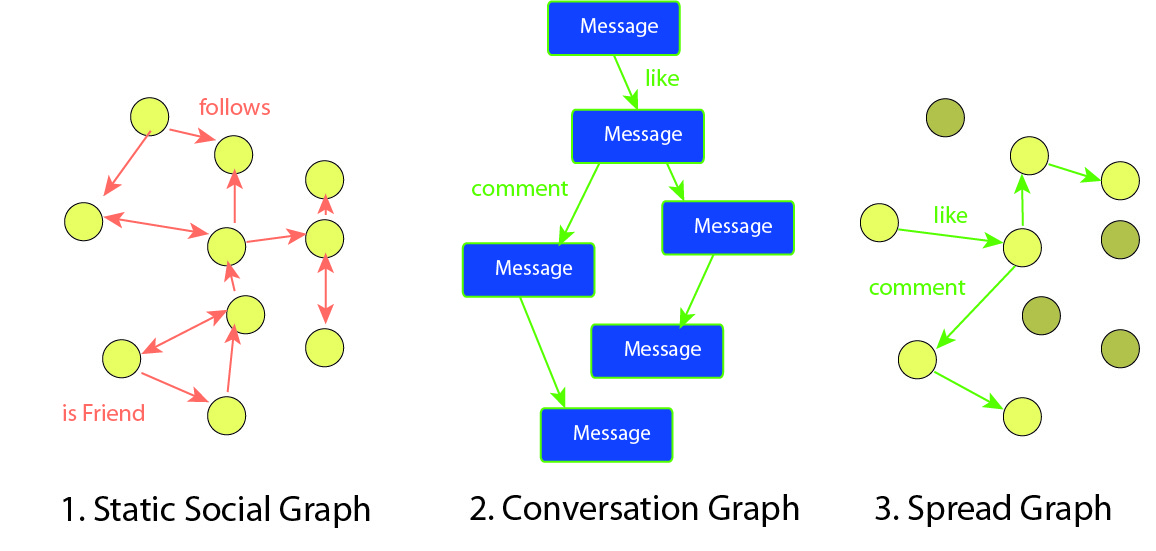
\includegraphics[width=6.2894in,height=3.0004in]{figures/chap3/chapitre3-img9.jpg}
    \caption[3 modèles de réseau]{Les 3 types de graphe classiquement extraits des données de réseaux sociaux}
\end{figure}

Plusieurs types de graphes peuvent \^etre extraits :

\begin{itemize}
\item \textbf{Graphe social statique}: représentant les relations pré-existantes dans la structure du réseau étudié (untel est ami avec untel, untel suit untel, etc.)
\item \textbf{Graphe conversationnel}: représentant toutes les interactions qui entourent et structurent la diffusion de messages 
\item \textbf{Graphe de diffusion}: représentant les interactions qui se sont produites entre les acteurs durant \ la diffusion du message. Ce dernier type de graphe est un recoupement des deux autres.
\end{itemize}


Dans notre étude, le graphe social statique ne présente pas particulièrement d{\textquoteright}intér\^et puisqu{\textquoteright}il correspond à un ensemble de relations peu affecté par les discussions. De plus, nous ne disposons dans le jeu de données Weiboscope que de son état final qui ne témoigne pas de l{\textquoteright}évolution des relations. Nous voulons obtenir ici les graphes de diffusion sous la forme de conversations structurées\textbf{~(}graphe directionnelle des \ réponses et commentaires) de l{\textquoteright}ensemble des messages. Dans un article paru dans \textit{Nature} \citep{Weng2012}, les chercheurs du \textit{Centre de Recherche sur les Systèmes Complexes} de l{\textquoteright}Université d{\textquoteright}Indiana identifient les caractéristiques des mèmes connaissant le plus de succès (la plus large diffusion). Un travail de visualisation de mèmes identifiés par des hashtags sur Twitter leur permet notamment de mettre à jour des motifs particuliers dans la structure des conversations.


\begin{figure}[ht]
    \centering
    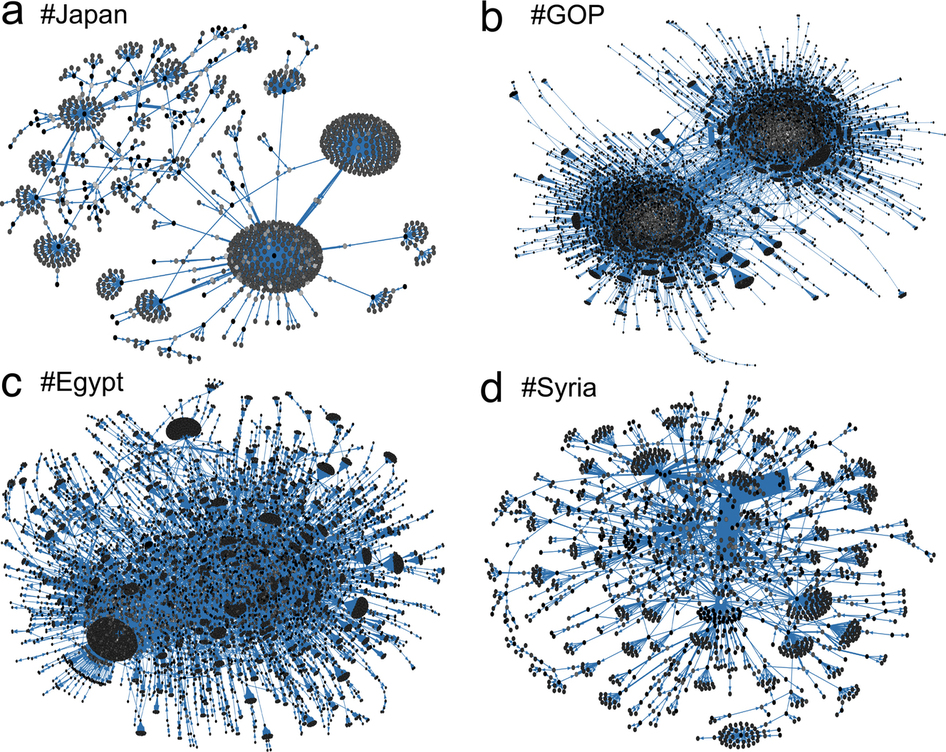
\includegraphics[width=5.5669in,height=4.4224in]{figures/chap3/chapitre3-img10.jpg}

    Nodes represent Twitter users, and directed edges represent retweeted posts that carry the meme. The brightness of a node indicates the activity (number of retweets) of a user, and the weight of an edge reflects the number of retweets between two users. \newline
    (a) The \textit{\#Japan}  meme shows how news about the March 2011 earthquake propagated. \newline
    (b) The \textit{\#GOP} tag stands for the US Republican Party and as many political memes, displays a strong polarization between people with opposing views. \newline
    Memes related to the Arab Spring and in particular the 2011 uprisings in (c) \textit{\#Egypt} and (d) \textit{\#Syria} display characteristic hub users and strong connections, respectively.
    
    \caption{Graphe de diffusion de hashtags sur Twitter d{\textquoteright}après \citep{Weng2012} }

\end{figure}


Nous avons mené un travail préliminaire afin de mener plusieurs expérimentations sur la visualisation de graphes conversationnels. Après avoir identifié quelques-uns des hashtags les plus discutés de l{\textquoteright}année 2012 sur Sina Weibo (voir la section \ref{sec:hashtags}), nous avons procédé à la visualisation des échanges pour chacun d'entre eux. Afin de mettre à jour le graphe conversationnel entourant les hashtags sélectionnés sur Sina Weibo, nous avons choisi d{\textquoteright}extraire la séquence d{\textquoteright}interactions des messages (mentions, retweets) composant chaque mème (voir algorithme \ref{algo:hashtags-graph}.

\begin{figure}
    
    \label{algo:hashtags-graph}
    % Hashtags
    \begin{algorithm}[H]
        \caption{Hashtags conversational graphs}
        \label{algo:hashtags-graph}
        \begin{algorithmic}
            \Require{$M$ is a set of microblog messages}
            \State $H(h,Gh)$ is a set of all hashtags conversational graphs

            \Function{HashtagsGraph}{$M$}
                \For{message $m$ in $M$}

                    \If{hashtag $h$ in $m$} 
                        \State $Gh=(Vh,Eh)$ is $h$ conversational graph
                        \If{ quotes or rt $e(userA,userB)$ in $m$}
                            \State $Eh \gets e(userA,userB)$ and $Vh \gets userA,userB $
                        \EndIf
                        \State $H \gets (h,Gh)$ 
                    \EndIf
                \EndFor
            \EndFunction
        \end{algorithmic}
    \end{algorithm}
    \caption{Algorithme pour constituer les graphes conversationnels des hashtags d'après un ensemble de message}
\end{figure}

Cette structure de graphe nous permet de représenter la diffusion de chaque mème sous forme d{\textquoteright}un graphe contenant un node par utilisateur et un ensemble de relations correspondant aux échanges visibles dans les textes des messages. Dans un premier temps, le logiciel \textit{Graphviz }nous a permis d{\textquoteright}obtenir une représentation basique du graphe conversationnel afin d{\textquoteright}avoir un aper\c{c}u sur la nature des conversations par l{\textquoteright}observation des motifs qui la compose. En effet, si les deux mesures identifiées à l{\textquoteright}étape précédente (volume de messages et \ volume d{\textquoteright}échanges) nous permettent d{\textquoteright}effectuer un premier tri parmi les hashtags, cette première visualisation nous permet de considérer la nature des échanges et l{\textquoteright}implication des utilisateurs d{\textquoteright}après la structure des motifs conversationnels. Chaque utilisateur est symbolisé par un point et chaque message par un trait reliant deux utilisateurs. Un motif très compact reflète une conversation animée entre des utilisateurs peu nombreux échangeant beaucoup. A l{\textquoteright}inverse, un motif disparate reflète des échanges plus brefs et morcelés.

\begin{figure}[ht]
    
    \begin{minipage}[b]{0.4\linewidth}
        \centering
        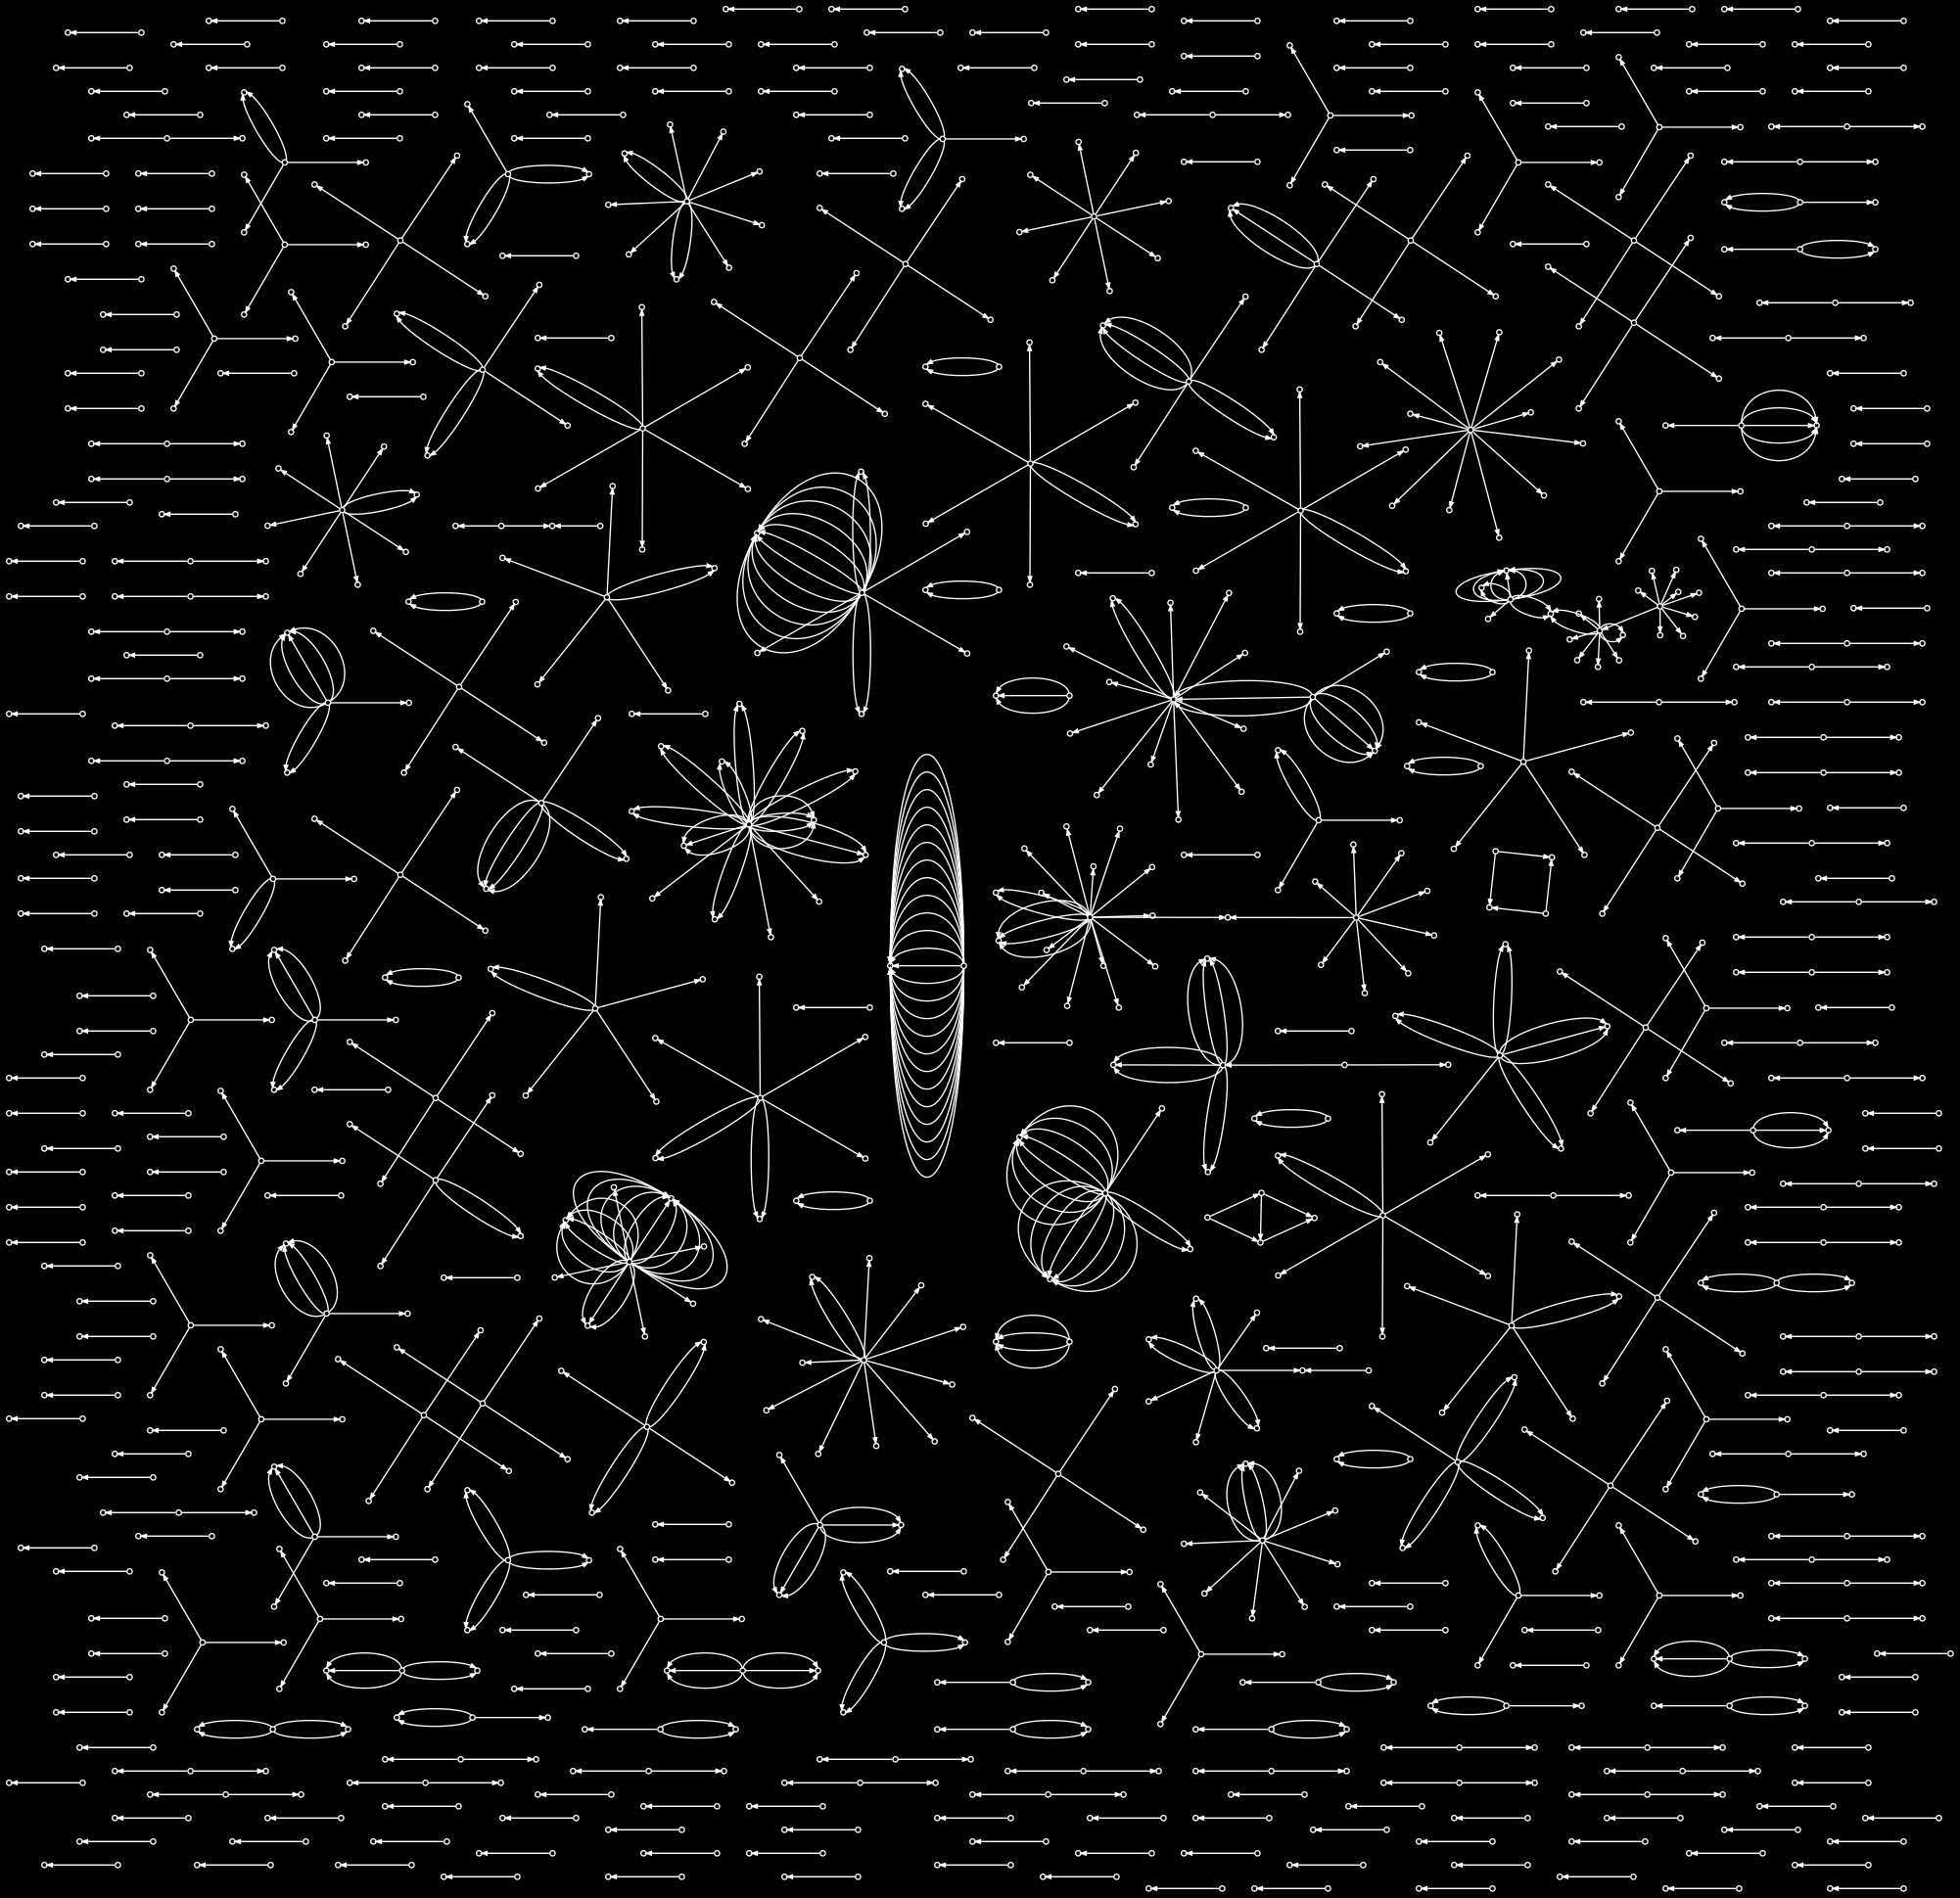
\includegraphics[width=2.5in,height=2.5in]{figures/chap3/chapitre3-img11.png}
        \par\vspace{0pt}
    \end{minipage}
    \begin{minipage}[b]{0.55\linewidth}
        \centering
        \raggedright
        \textit{WeicoPlus }est une application mobile permettant
        d{\textquoteright}utiliser Sina Weibo. Le hashtag \#WeicoPlus\# est
        ajouté automatiquement quand les utilisateurs postent des photos
        depuis ce service. 

        Ainsi, on remarque que le graphe conversationnel
        entourant WeicoPlus se compose essentiellement de messages simples,
        mais ne donne pas lieu à une conversation structurée - à
        l{\textquoteright}exception de quelques rapides échanges entre un
        nombre réduit de personnes.
        \par\vspace{0pt}
    \end{minipage}

    \caption[Visualisation simple du hashtag{\textquotedblleft}WeicoPlus{\textquotedblright}] {Fig. Visualisation simple du hashtag{\textquotedblleft}WeicoPlus{\textquotedblright}, un trait représente un échange entre deux utilisateurs}
\end{figure}


\begin{figure}[ht]
    \begin{minipage}[b]{0.4\linewidth}
        \centering
        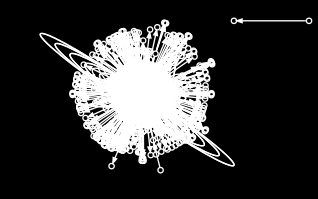
\includegraphics[width=2.5in,height=1.5in]{figures/chap3/chapitre3-img12.png}
        \par\vspace{0pt}
    \end{minipage}
    \begin{minipage}[b]{0.55\linewidth}
        \centering
        \raggedright
        A l{\textquoteright}inverse, le hashtag {\textquotedblleft}Veuve
        d{\textquoteright}enfant
        unique{\textquotedblright} \zh{\#失独母亲\#} cristallise
        le débat en une forme très dense qui reflète une surenchère de
        commentaires et d{\textquoteright}actions autour du hashtag, propre
        d{\textquoteright}une conversation animée. 
        \par\vspace{0pt}
    \end{minipage}

    \caption[Visualisation simple des conversations autour du hashtag Veuve d{\textquoteright}enfant unique]{Visualisation simple des conversations autour du hashtag Veuve d{\textquoteright}enfant unique}
\end{figure}

Les différents modèles de conversation que nous obtenons dans cette première étape se présentent sous une forme schématique et peu détaillée. Afin de comprendre plus en détails les dynamiques conversationnelles qui les entourent, nous avons choisi de sélectionner trois exemples parlants de hashtags dont les graphes conversationnels présentent des particularités des modèles de diffusion dissemblables et organisés. Pour chacun d{\textquoteright}eux, nous allons procéder à une analyse plus détaillée des graphes conversationnels afin de considérer les différences entre ces différents modèles.

% \begin{figure}[th]
%     \centering
%     \subfloat[Pluie torrentielle à Tianjing]{
%         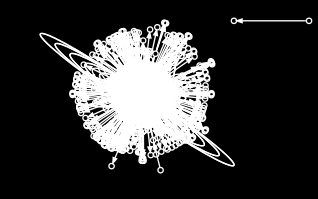
\includegraphics[width=2.3224in,height=1.4449in]{figures/chap3/chapitre3-img13.png}
%     }

%     \subfloat[Veuve à l{\textquoteright}enfant unique]{
%         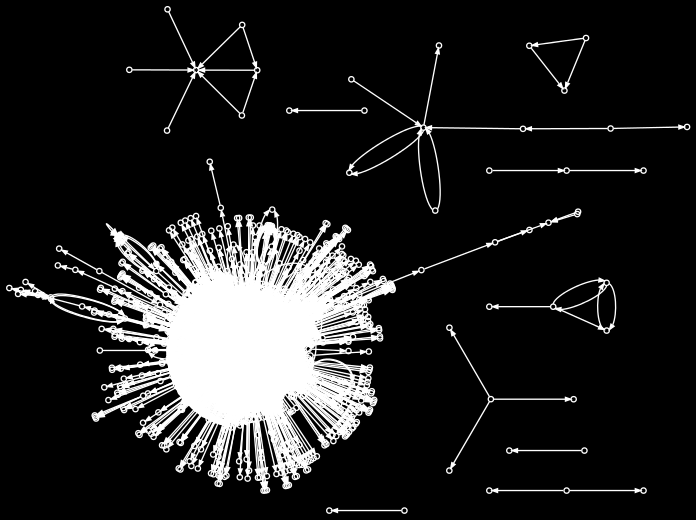
\includegraphics[width=2.3004in,height=1.7224in]{figures/chap3/chapitre3-img14.png}
%     }

%     \subfloat[Abolition des lois sur la prostitution]{
%         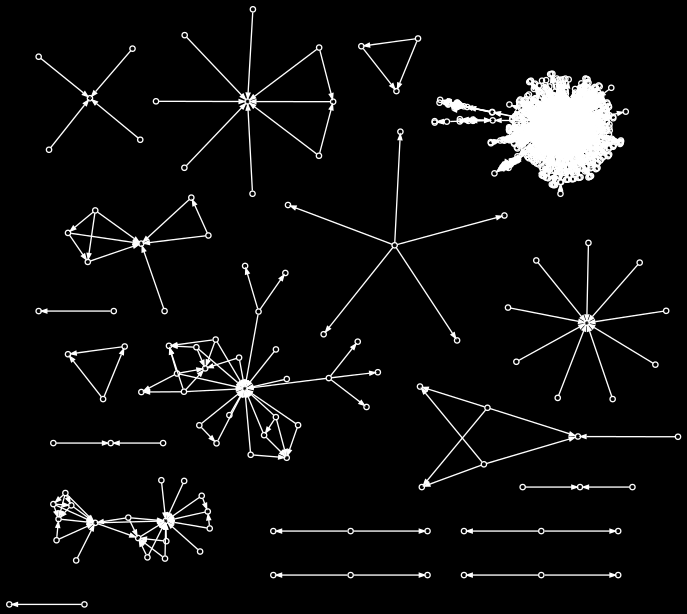
\includegraphics[width=2.1449in,height=1.9224in]{figures/chap3/chapitre3-img15.png}   
%     }
  
%     \caption{Visualisation des conversations autour de trois hashtags}
% \end{figure}


Nous voyons que les trois représentations des graphes ci-dessus donnent à voir des structures plus ou moins morcelées, avec un ensemble de points et de lignes très compactes qui représentent la majeure partie de la conversation. Afin de visualiser plus précisément les groupes et les dynamiques qui constituent les discussions autour de chaque hashtag, nous allons utiliser le logiciel Gephi \citep{Bastian2009} afin d{\textquoteright}examiner de plus près la composition de ces graphes. Pour ce faire, Gephi va nous permettre d{\textquoteright} {\textquotedblleft}étaler{\textquotedblright} le graphe en repositionnant les nodes et en les coloriant pour en identifier les composantes et les tendances.

Chaque utilisateur est représenté sous la forme d{\textquoteright}un point. La taille des points correspond à l{\textquoteright}importance de l{\textquoteright}utilisateur dans le réseau total des échanges, caractérisé par son degré de centralité intermédiaire (\textit{betweenness centrality}), une mesure topologique correspondant au nombre de plus courts chemins du graphe passant par cet utilisateur. La couleur est utilisée pour représenter la \textit{modularité }du réseau, c{\textquoteright}est à dire le nombre de communautés engagées dans la conversation définies comme les cliques d{\textquoteright}utilisateurs constituant plus de 1\% du réseau total d{\textquoteright}échange \citep{Blondel2008}. La position des nodes est calculée gr\^ace à l{\textquoteright}algorithme \textit{Force Atlas 2} \citep{Bastian2009} utilisant une modélisation physique o\`u les nodes peu connectés entre eux se repoussent et ceux très connectés s{\textquoteright}attirent. Ainsi, la proximité de deux nodes sur le graphe témoigne d{\textquoteright}une proximité lors des conversations, c{\textquoteright}est à dire de l{\textquoteright}existence d{\textquoteright}un échange entre eux (citations, commentaires ou retweets). Pour davantage de visibilité, certaines conversations sub-alternes représentant moins de 1\% du total ont été effacées. Egalement, les nodes possédant un degré inférieur à 3 (moins d{\textquoteright}un échange avec au moins trois autres nodes du grahe) ne sont pas représentés.

\textbf{Exemple 1 : Pluie torrentielle à Tianjing}

Le premier mème choisi parle d{\textquoteright}une catastrophe naturelle, sous la forme d{\textquoteright}une pluie diluvienne qui s{\textquoteright}est abattue sur la ville de Tianjin durant la nuit du 21 au 22 Juillet 2012.

\begin{figure}[h!]
    \centering
    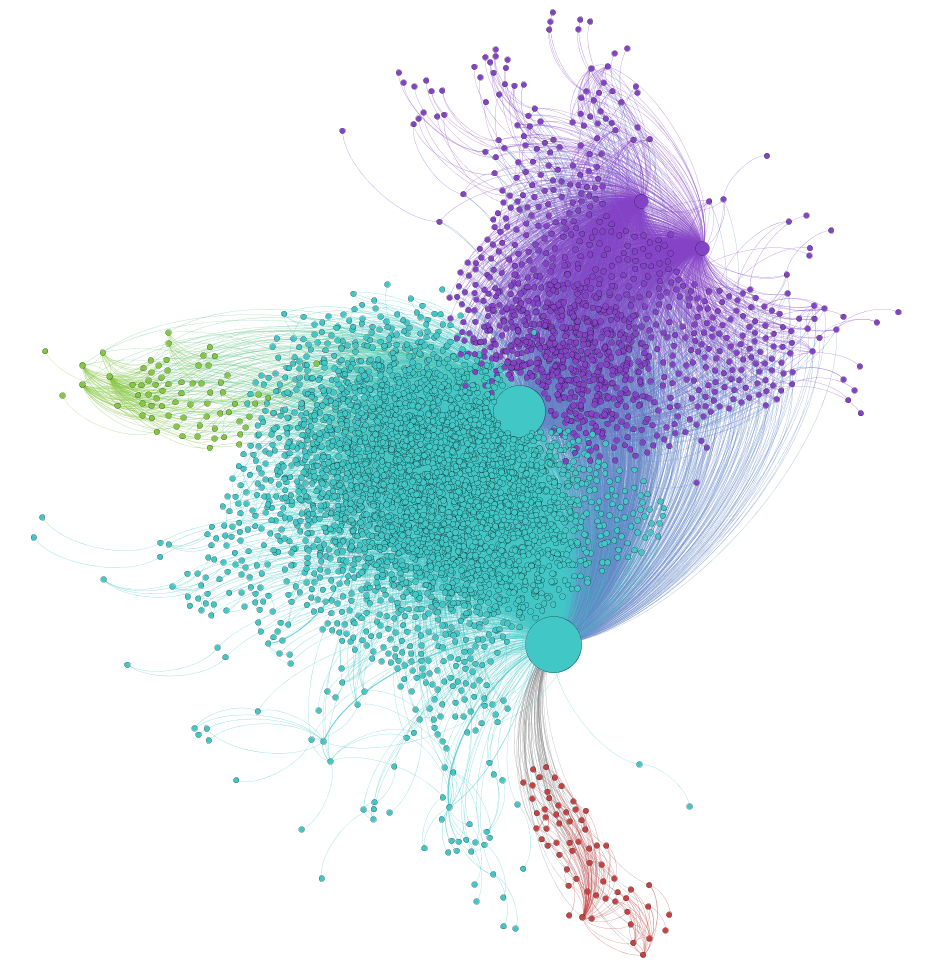
\includegraphics[width=6in,height=6in]{figures/chap3/chapitre3-img17.png}
    \caption{Exemple 1 : Tianjin Baoyu}
    \label{fig:graph-tianjin}
\end{figure}

Sur la figure \ref{fig:graph-tianjin}, on voit nettement 4 groupes constitués autour de gros diffuseurs (les nodes les plus gros) qui composent 85\% du graphe. Plusieurs groupes semblent s{\textquoteright}emparer de la conversation mais on voit peu d{\textquoteright}activité entre les nodes alors que les échanges se déroulent autour de quelques utilisateurs très centraux. Cela traduit le fait que peu de personnes ont réellement discuté l{\textquoteright}information et elles se sont simplement contentées de la relayer.


La diffusion d{\textquoteright}un fait divers très local (il se passe à Tianjing) est entrainée par peu de sources très importantes (les quelques nodes de grande taille), vraisemblablement des journaux et médias locaux qui annoncent la nouvelle (presse, photos-choc d{\textquoteright}innondations, etc). La conversation est peu active et très structurée, nous sommes en présence d{\textquoteright}un modèle classique de diffusion de masse.

\begin{figure}[h!]
    \centering
    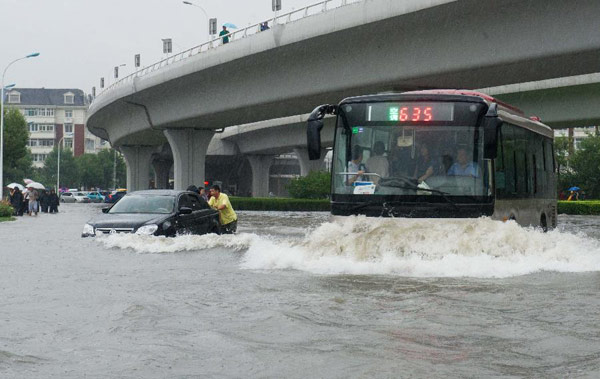
\includegraphics[width=4.76in,height=3in]{figures/chap3/chapitre3-img16.jpg}
    \caption[Photo de Tianjin durant la pluie torentielle en Juillet 2012]{\textit{Downpour bypasses Beijing, batters neighbor, }in Qinghua News le 2012-07-26 13:29:59, \url{http://news.xinhuanet.com/english/china/2012-07/26/c_131740415.htm} consulté le 27 Juin 2014.}
\end{figure}

\textbf{Exemple 2 : Veuve de l{\textquoteright}enfant unique}

Un autre sujet discuté par une très large quantité de personnes appara\^it sous le terme {\textquotedbl}\textit{shidu muqin}{\textquotedbl}, forme contractée signifiant \textit{{\textquotedblleft}mère qui a perdu son enfant unique{\textquotedblright}} (\zh{\#失独母亲\#}). Ce hashtag désigne un phénomène de société bien connu en Chine o\`u le deuil de la perte d{\textquoteright}un enfant se double souvent pour une mère chinoise seule de l{\textquoteright}absence de ressources pour vivre. En effet, l{\textquoteright}absence de système de retraite fait porter aux enfants la responsabilité de la survie de la famille.

\begin{figure}[h!]
    \centering
    
\includegraphics[scale=0.7]{figures/chap3/chapitre3-shidumuqin.jpg}
    \caption[Photo illustrative de Shidu Muqin]{\zh{一位失独母亲的独语} paru le 17 Juillet 2012 in \textit{Nandu Weekly} le 2012.07.17, \url{http://www.nbweekly.com/news/special/201207/30571.aspx}, consulté le 27 Juin 2014.}
    \label{fig:photo-shidumuqin}
\end{figure}


\newpage


Le graphe \ref{fig:shidumuqin} ici est fait de deux grands groupes composant à eux deux près de 95\% du graphe total. Les discussions sont très polarisées et menées par peu de participants (les nodes les plus gros sur le graphe). Peu de personnes très influentes concentrent les discussions autour d{\textquoteright}eux, accompagnés ou suivis d{\textquoteright}une foule de commentateurs.  

\begin{figure}[h!]
    \centering
    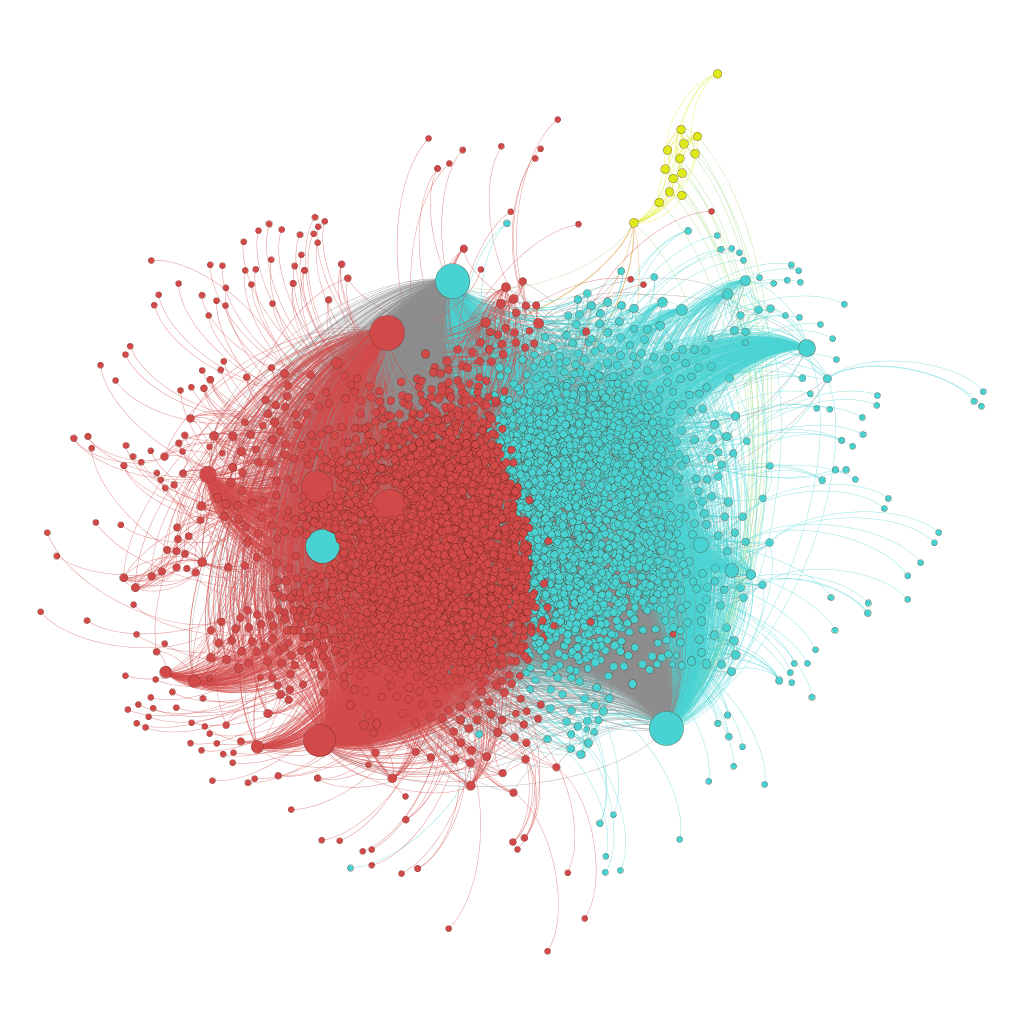
\includegraphics[width=6.0114in,height=6.0114in]{figures/chap3/chapitre3-img18.png}
    \caption{{\textquotedblleft}Shidu Muqin{\textquotedblright}}
    \label{fig:shidumuqin}
\end{figure}



Cet exemple donne à voir des groupes bien définis et très proches o\`u plusieurs acteurs majeurs mènent la discussion. Les dynamiques d{\textquoteright}échanges autour d{\textquoteright}une question de société (la loi de l{\textquoteright}enfant unique en Chine et ses conséquences) s{\textquoteright}articule en groupes distincts sans pour autant amener à des controverses importantes (qui se traduiraient par des discussions longues et houleuses). Ici, les leaders d{\textquoteright}opinion font la discussion et la diffusion se fait au travers d{\textquoteright}eux.

\clearpage
\textbf{Exemple 3 : Abolition des lois sur la prostitution}

Le hashtag \textit{{\textquotedblleft}Abolissons la loi piaowudong nuzui{\textquotedblright} }est l{\textquoteright}expression d{\textquoteright}une campagne pour l{\textquoteright}abolition d{\textquoteright}une législation scandaleuse sur la prostitution en Chine. Depuis les années 80, la loi chinoise interdit la prostitution et prévoit la condamnation des deux parties qui s{\textquoteright}adonnent à un échange d{\textquoteright}argent. Baptisé \textit{{\textquotedblleft}Piaowudong nuzui{\textquotedblright}, }cette loi a vu plusieurs cas absurdes impliquant des viols organisés sur mineurs se solder par la condamnation et l{\textquoteright}emprisonnement des enfants incriminés. Relayés par les journalistes, les scandales à répétition ont éclatés à plusieurs reprises, impliquant parfois des officiels du Parti souvent blanchis alors que des enfants étaient eux emprisonnés. 

\begin{figure}[th]
    \centering
    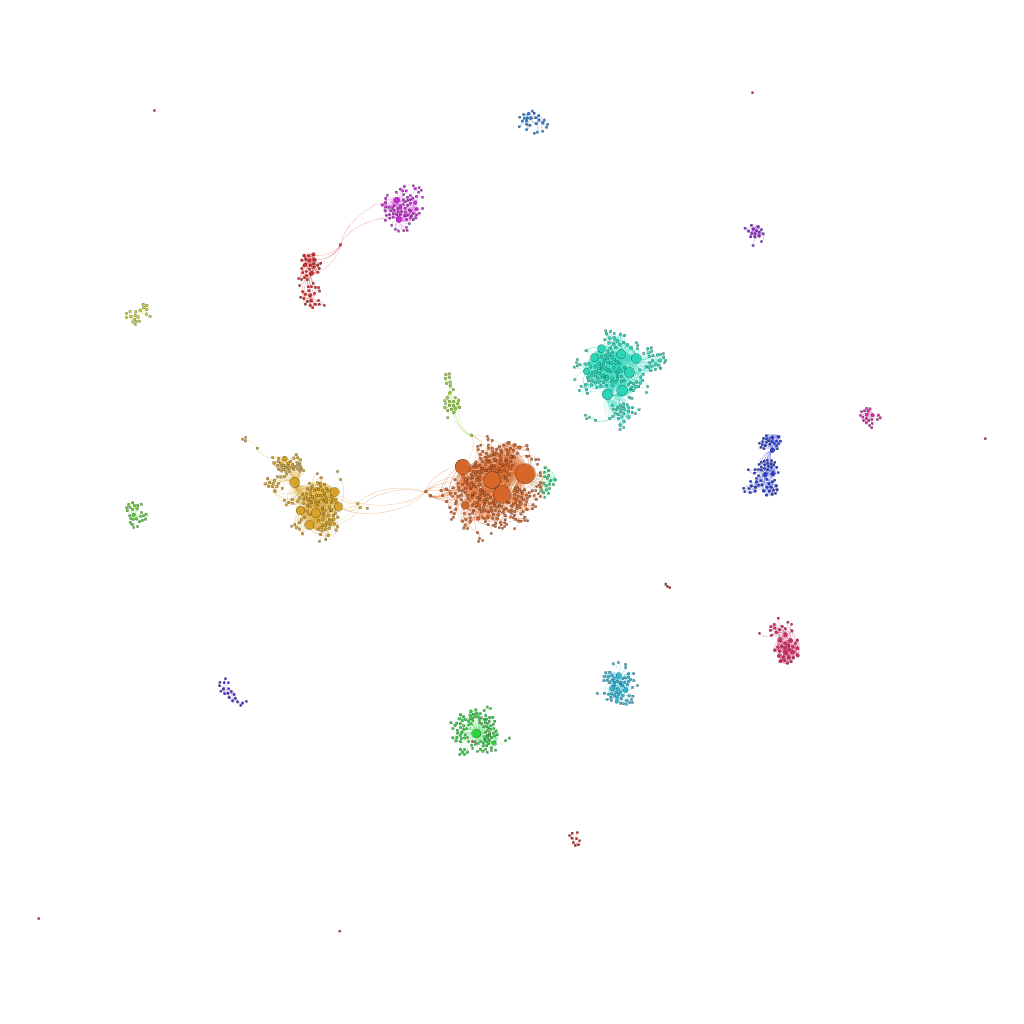
\includegraphics[width=6.0114in,height=6.0114in]{figures/chap3/chapitre3-img19.png}
    \caption{ {\textquotedblleft}Piaowudong nuzui{\textquotedblright}}
    \label{fig:piaodong}
\end{figure}

Le graphe \ref{fig:piaodong} des discussions autour de l{\textquoteright}abolition de cette loi montre que de nombreux groupes discutent séparément de cette question puisque les premiers 50\% du graphe sont déjà constitués de plus d{\textquoteright}une quinzaine de clusters. Les groupes sont très éloignés entre eux, n{\textquoteright}entretenant que peu de relations et connaissant une activité intense.


Cet exemple présente les caractéristiques d{\textquoteright}une conversation très décentralisée dans laquelle de nombreux acteurs différents prennent part. L{\textquoteright}émergence de ce type de discussion fragmentée témoigne d{\textquoteright}un usage particulier de la discussion sur le réseau social et montre comment la discussion autour d{\textquoteright}un sujet peut s{\textquoteright}étendre sans afficher de relations directes dans le média lui-m\^eme. Ici un agent extérieur (en l{\textquoteright}occurence un article du journal \textit{Nanfang Zhoumo }sur le sujet) fait na\^itre la conversation sans pour autant l{\textquoteright}accaparer et la centraliser. Plus difficilement détectable et contr\^olable, cette dernière configuration est typique du mème car elle se développe de fa\c{c}on large et durable entre des groupes à l{\textquoteright}origine peu connectés.


\bigskip

Cette première visualisation des graphes conversationnels nous permet d{\textquoteright}explorer quelques types précis d{\textquoteright}échanges et d{\textquoteright}en proposer une première lecture. Néanmoins, le procédé de visualisation reste rudimentaire et soulève plusieurs questions que nous nous donnons pour t\^ache de continuer à explorer. Premièrement, dans quel espace a lieu cette représentation? En étalant ainsi ces graphes conversationnels, quelle action réalisons-nous réellement et quelle en est la valeur pour l{\textquoteright}analyse? à plus forte raison, quelle est la relation de cette espace du graphe conversationnel avec les autres formes d{\textquoteright}espace, et plus notamment l{\textquoteright}espace du réel géographique et l{\textquoteright}espace de la représentation par le langage?

Nous souhaitons ici mettre en perspective ces différentes dimensions afin d{\textquoteright}enrichir le modèle d{\textquoteright}étude. En effet l{\textquoteright}analyse de la diffusion utilise principalement les graphes des réseaux de diffusion mettant en scène les utilisateurs et leurs interactions en ligne. Loin d{\textquoteright}\^etre inintéressant, ce type de schéma est néanmoins très réducteur car il se fonde sur un modèle communicationel très primaire \textit{{\textquotedblleft}émetteur-récepteur{\textquotedblright} }dont on conna\^it les limites. Les travaux de Jacobson ont notamment permis d{\textquoteright}étoffer ce modèle en considérant les différents aspects fonctionels des actes de communication.


\begin{figure}[h!]
    \centering

    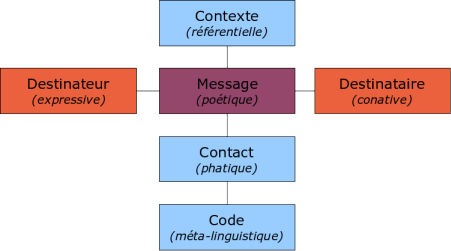
\includegraphics[width=4.6894in,height=2.6114in]{figures/chap3/chapitre3-img5.png}

    \caption[Modèle de Jakobson]{ Le modèle de Jakobson présente différents aspects des actes de communication que nous pouvons chercher à adapter dans le contexte des échanges en ligne.}

\end{figure}

Ainsi, en nous basant sur les modèles des théories de la communication, nous pouvons peut-\^etre améliorer les modèles méthodologiques d{\textquoteright}analyse. Nous proposons ici la notion de \textit{topogramme }comme modèle pour comprendre les motifs de diffusion des mèmes, considérés comme \textit{topos} ou \textit{lieux communs. }Le topogramme, en tant que représentation graphique des différentes dimensions et dynamiques lisibles dans les données nous permet donc d{\textquoteright}approcher un travail \ d{\textquoteright}observation précise de la diffusion des mèmes, voire par la suite de classification des actes de communication en ligne. Afin de prendre en compte, les différents aspects de la communication, il nous faut donc effectuer une analyse à plusieurs niveaux (multi-layers), regroupant un ensemble de réseaux à la fois sémantique, conversationnel et géographique.